\documentclass[12pt,a4paper]{article}

% ==================== 基础包 ====================
\usepackage[UTF8]{ctex}                     % 中文支持
\usepackage{geometry}                       % 页面设置
\usepackage{graphicx}                       % 图片插入
% （已删除 svg 包：所有流程图已转为 PNG）
\usepackage{booktabs}                       % 三线表
\usepackage{multirow}                       % 表格合并
\usepackage{array}                          % 表格增强
\usepackage{amsmath,amssymb}                % 数学公式
\usepackage{hyperref}                       % 超链接
\usepackage{caption}                        % 图表标题
\usepackage{subcaption}                     % 子图
\usepackage{xcolor}                         % 颜色
\usepackage{minted}                         % 代码高亮（替代 listings，支持 UTF-8）
\usepackage{enumitem}                       % 列表定制
\usepackage{fancyhdr}                       % 页眉页脚
\usepackage{setspace}                       % 行距
\usepackage{tikz}                           % 简单框图
\usepackage{colortbl}                       % 表格颜色
\usepackage{float}                          % [H] 强制不浮动

% ==================== 图片路径配置 ====================
\setlength{\headheight}{14pt}
\addtolength{\topmargin}{-2pt}

% ==================== 页面设置 ====================
\geometry{left=2.2cm,right=2.2cm,top=2.5cm,bottom=2.5cm}
\setstretch{1.5}
\setlength{\parindent}{2em}
\setlength{\parskip}{0.5em}

% ==================== 图表设置 ====================
\graphicspath{{photo/}}
\captionsetup{font=small,labelfont=bf,skip=5pt}

% ==================== 代码高亮 ====================
\setminted{
    fontsize=\small,
    frame=single,
    linenos=true,
    breaklines=true,
    python3=true,
}

% ==================== 页眉页脚 ====================
\pagestyle{fancy}
\fancyhf{}
\fancyhead[C]{\small 视觉认知工程课程大作业}
\fancyfoot[C]{\thepage}

% ==================== 标题信息 ====================
\title{\textbf{基于脑启发核心集选择的轻量级 VLA 机械臂动作预测}}
\author{杜辰宇 \hspace{2cm} U202315265}
\date{\today}

\begin{document}

\maketitle
\thispagestyle{empty}

% ==================== 摘要 ====================
\begin{abstract}
视觉-语言-动作（VLA）模型的训练面临严重的数据冗余问题：时序冗余与分布冗余导致模型在大量低信息帧上浪费算力，同时过拟合于常见模式。本文从"冗余如何定义"这一根本问题出发，受大脑信息筛选机制启发，系统探索了五种冗余定义方式——分布冗余、事件分割、预测编码、压缩冗余与几何覆盖冗余——并验证了每种定义与数据特性的匹配度。在 ALOHA Sim Transfer Cube 数据集上，本文提出的密度过滤最远点采样（Density-Filtered FPS）方法以仅 10\% 的训练数据达到 Test MSE = \textbf{0.003792}，较随机基线（0.007229）降低 \textbf{47.5\%}。关键发现：单一全局最优方法的信息完整性无法通过任何分层、加权或互补的融合策略复现，18 个融合实验无一超越单一最优。本文的否定性验证（时序方法、自编码器方法、多种融合均失败）恰恰证明：冗余的定义必须与数据特性和目标任务高度匹配。
\end{abstract}

\newpage
\tableofcontents
\newpage

% ==================== 1. 引言与背景机制调研 ====================
\section{引言与背景机制调研}
\label{sec:intro}

\subsection{VLA 模型与数据冗余困境}

视觉-语言-动作（Vision-Language-Action, VLA）模型是当前具身智能领域的核心研究方向，负责将视觉感知与自然语言指令映射为精确的机械臂动作序列\cite{zhao2023act}。从 ACT（Action Chunking with Transformers）到 OpenVLA\cite{kim2024openvla}，VLA 模型在模仿学习任务中展现出强大的端到端学习能力。然而，真实 VLA 训练面临严峻的"数据冗余与算力墙"困境：

\begin{itemize}[leftmargin=2em]
    \item \textbf{时序冗余}：相邻帧视觉变化微小，动作几乎不变，模型在大量"发呆帧"上浪费梯度；
    \item \textbf{分布冗余}：某些简单动作在特征空间高度聚集，过度采样导致模型过拟合于常见模式；
    \item \textbf{次优噪声}：特征空间边缘的孤立点可能是传感器噪声，教学价值为零。
\end{itemize}

以本文使用的 ALOHA Sim Transfer Cube 数据集为例，50 个成功演示轨迹约 20,000 帧，其中大量帧对应"夹爪空移""悬停等待"等低信息状态。直接在全量数据上训练不仅消耗巨大算力，还会导致模型泛化能力下降。核心集选择（Coreset Selection）——从海量数据中筛选最具信息价值的高质量子集——成为解决这一困境的关键路径\cite{sorscher2022beyond}。

\subsection{脑启发核心集选择机制}

大脑在信息处理中展现出惊人的筛选效率：视网膜每秒接收约 $10^9$ 比特信息，而意识仅能处理约 $10^2$ 比特。这种高效筛选并非随机丢弃，而是基于预测价值、信息密度与任务相关性的主动选择。本文将五种脑机制映射为核心集选择算法（表~\ref{tab:brain_mapping}）。

\begin{table}[htbp]
\centering
\caption{脑机制到核心集选择算法的映射}
\label{tab:brain_mapping}
\small
\begin{tabular}{@{}lp{5.5cm}p{4.0cm}p{2.8cm}@{}}
\toprule
\textbf{脑机制} & \textbf{生物学原理} & \textbf{算法映射} & \textbf{冗余定义} \\
\midrule
预测编码 & 大脑基于先验预期生成感官预测，预测一致时神经活动被抑制 & 滑动窗口线性回归预测误差 & 低预测误差 = 时序冗余 \\
RAS 网状激活 & 过滤背景噪音，聚焦高信息效用刺激 & K-Means 稀疏簇偏好 + 动态保底 & 过度聚集 = 分布冗余 \\
事件分割 & 行为转换时刻分配更多注意力资源 & 动作变化率检测 + 事件边界保底 & 低动作变化率 = 时序冗余 \\
意外检测 & 对"看不懂"的刺激分配注意力 & 自编码器重建误差 & 重建误差小 = 压缩冗余 \\
海马体空间编码 & 海马体 place cell 编码空间位置的几何关系 & 最远点采样（FPS）+ 密度过滤 & 远且不孤立 = 几何冗余 \\
\bottomrule
\end{tabular}
\end{table}

上述五种脑机制为本文的冗余定义提供了生物学层面的理论基础。\textbf{预测编码理论}（Predictive Coding）认为，大脑本质上是一个预测机器：神经元持续对世界进行前向预测，只有当感官输入打破预测时才会产生显著的信号更新\cite{millidge2021predictive}。这意味着，高度可预测的连续帧对应大脑中的"低更新状态"，在训练数据中即为时序冗余。\textbf{RAS 网状激活系统}则负责从海量感官输入中筛选高信息效用的部分，类似于特征空间中稀疏簇的优先选择：过度聚集的簇对应"背景噪音"，稀疏簇对应"前景信号"。\textbf{事件分割}由海马体支持，人类会自动将连续行为切分为离散事件，事件边界处分配更多记忆资源。\textbf{意外检测}机制使大脑对无法内化的刺激保持敏感，自编码器重建误差正是这一机制的量化实现。\textbf{海马体空间编码}则是本文最新引入的脑机制映射：海马体中的 place cell 通过几何位置关系编码空间信息，对应特征空间中的最远点采样——优先选择距离已选集合最远的点，以保证空间覆盖的完整性。

然而，将这些脑机制直接翻译为算法并不总是有效。大脑进化出的信息筛选策略是针对自然场景的通用解决方案，而机器人模仿学习面对的是高度结构化的单任务数据。这种"机制—数据"的匹配度差异，正是本文大量否定性验证（时序方法、AE 方法、融合方法失败）的根源。

\subsection{脑机制映射框架图}

图~\ref{fig:brain_framework}展示了五种脑机制到核心集选择算法的完整映射链。每一条链路都包含"脑机制 $\rightarrow$ 冗余定义 $\rightarrow$ 算法实现 $\rightarrow$ 实验结果"四个环节。可以清晰看到：RAS 网状激活对应的分布冗余路径与海马体空间编码对应的几何冗余路径成功（MSE 分别为 0.003835 和 0.003792），而事件分割、压缩冗余路径均告失败，预测编码路径有效但有限。这一框架直观地说明，脑机制本身并不保证算法有效——关键在于冗余定义是否与数据特性匹配。

\begin{figure}[htbp]
    \centering
    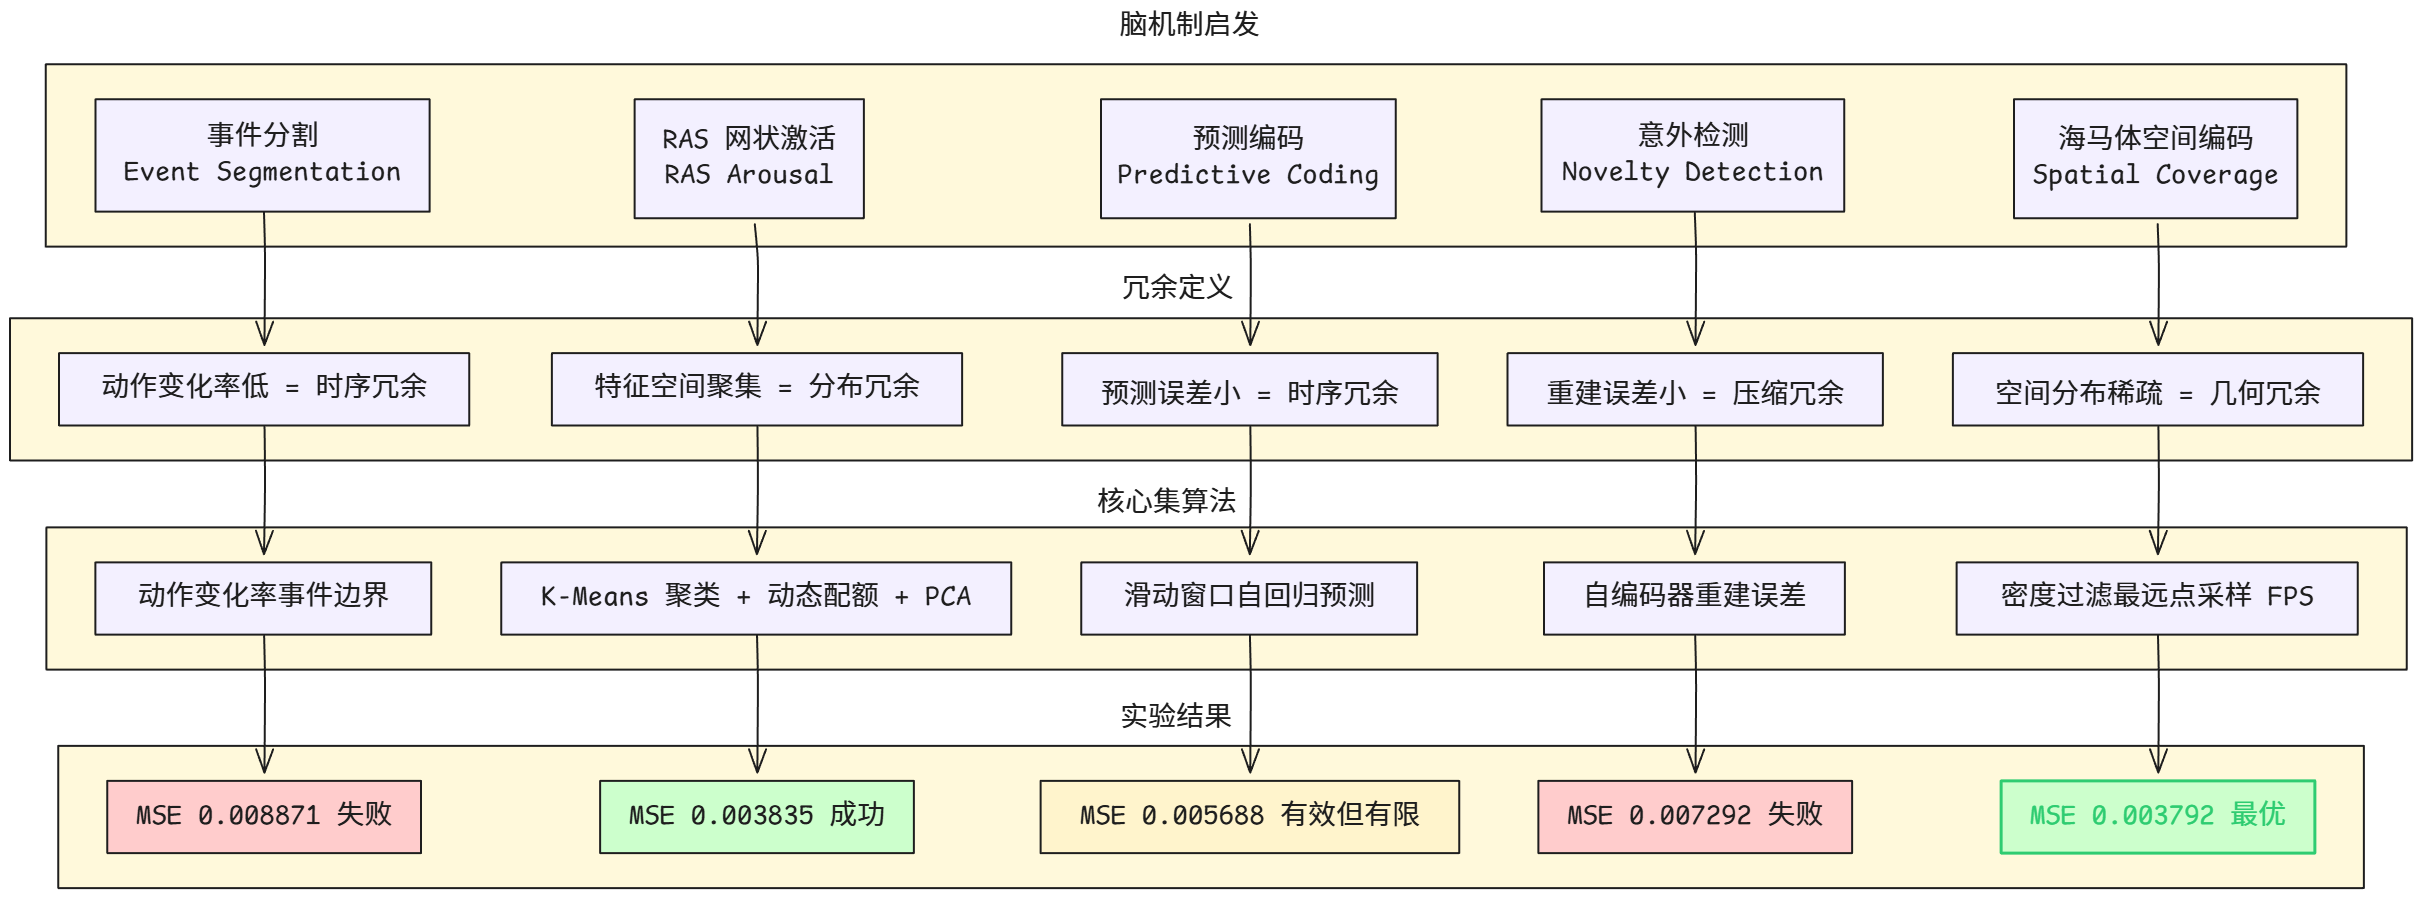
\includegraphics[width=1.0 \textwidth]{figF_brain_framework.png}
    \caption{脑机制到核心集算法的映射框架（五种方法全对齐）}
    \label{fig:brain_framework}
\end{figure}

\subsection{本文贡献}

本文的核心贡献在于从"冗余如何定义"出发，系统探索了脑启发机制在核心集选择中的适用边界，并揭示了核心集选择的深层规律：

\begin{enumerate}[leftmargin=2em]
    \item \textbf{系统性的核心集选择探索框架}：从五种脑启发的冗余定义出发（分布冗余、时序事件分割、预测编码、压缩冗余、几何覆盖冗余），独立设计并验证了对应的核心集选择算法，并进一步探索了多种融合策略。实验揭示了冗余定义与数据特性匹配度对最终性能的决定性作用——并非所有脑启发的机制都能直接转化为有效算法；
    \item \textbf{密度过滤 FPS 最优算法}：提出了密度过滤 FPS 方法，通过最远点采样保证特征空间的几何覆盖，并以 k-NN 局部密度估计温和修正边缘噪声点。该方法以仅 10\% 数据达到 Test MSE 0.003792，较随机基线降低 47.5\%，为全局最优；
    \item \textbf{融合实验揭示的深层规律}：设计了 18 组融合实验（5 种架构 $\times$ 多种参数配置），全部未能超越单一最优。分析表明，核心集选择中的"信息漏斗效应"与"信号相关性上限"使得简单融合无法产生信息增益，揭示了单一全局最优的深层合理性。
\end{enumerate}

% ==================== 2. 数据集与实验设置 ====================
\section{数据集与实验设置}
\label{sec:dataset}

\subsection{ALOHA Sim Transfer Cube 数据集}

实验在 ALOHA Sim Transfer Cube 数据集上进行\cite{zhao2023act}，包含 50 个成功的人类演示轨迹（Episodes），总计约 20,000 帧。每帧包含：多视角相机图像、末端执行器姿态、14DoF 联合动作标签。本文降维实验仅提取 top 视角摄像头与单臂 7DoF 动作（位置 3d + 旋转 4d）。数据划分采用 Episode 级别随机切分：80\%（40 Episodes，约 16,000 帧）用于训练集筛选，20\%（10 Episodes，约 4,000 帧）作为固定测试集，随机种子为 42。

\subsection{特征提取与模型设置}

\textbf{前端网络}：CLIP ViT-B/32（冻结权重）\cite{radford2021clip}，视觉特征 768d，文本特征 512d，拼接为 1280d 输入向量。基于 ResNet-18 的初步实验验证了核心集选择思路的有效性\cite{he2016resnet}，为进一步体现多模态融合优势，后续升级至 CLIP 视觉-语言对齐特征。

\textbf{预测模型}：四层 MLP（$1280 \rightarrow 512 \rightarrow 256 \rightarrow 128 \rightarrow 7$），ReLU 激活，Dropout=0.1，Xavier 初始化。Adam 优化器，初始学习率 $10^{-3}$，ReduceLROnPlateau 学习率衰减（factor=0.5, patience=5），早停 patience=15。

\textbf{公平性控制}：所有实验组使用同样的 MLP 结构、同样的超参数、同样的训练/测试划分。唯一变量：训练数据的筛选方式。Baseline 为随机抽取 10\% 训练帧（1,600 帧），运行 5 次取平均 Test MSE = 0.007229 $\pm$ 0.000963。

% ==================== 3. 核心集选择算法设计 ====================
\section{核心集选择算法设计：对"冗余"定义的独立思考}
\label{sec:coreset}

本章从五个维度定义冗余，系统验证每种定义与数据特性的匹配度。每节遵循统一结构：核心假设 $\rightarrow$ 脑机制映射 $\rightarrow$ 算法设计 $\rightarrow$ 实验结果 $\rightarrow$ 失败/成功原因分析。这是本文的核心创新所在。

% -------------------- 3.1 分布冗余 --------------------
\subsection{冗余定义一：分布冗余（K-Means + PCA 视角）}
\label{sec:distribution}

\textbf{核心假设}：视觉特征空间中过度聚集的帧 = 分布冗余。某些简单动作（如夹爪空移、悬停等待）在特征空间中高度聚集，过度采样会导致模型过拟合于常见模式，忽略稀疏但关键的状态（如夹爪开合瞬间）。

\textbf{脑机制映射}：RAS 网状激活系统 $\rightarrow$ 稀疏簇偏好。RAS 根据刺激的新奇度和任务相关性过滤信息，忽略重复的背景噪音。对应到算法：将视觉特征空间视为大脑的感觉皮层表征，K-Means 聚类划分不同的"感知模式"，稀疏簇对应少见但高信息效用的刺激，应被优先保留。

% ===== 图A：自适应聚类筛选算法流程 =====

\textbf{算法设计}（图~\ref{fig:kmeans_flow}）：输入 768d CLIP 视觉特征（16,000 帧）。

\textbf{Step 1：PCA 去噪}（v1.1+ 配置）。将 768d 特征投影至 400d 子空间，保留 99.8\% 方差。PCA 变换去除了干扰 K-Means 聚类的噪声方向。

\textbf{Step 2：K-Means 聚类}。将降维后特征聚为 $k = \lfloor 1600 / 3 \rfloor = 533$ 个簇，使用 k-means++ 初始化，最大迭代 300 次。

\textbf{Step 3：多样性得分计算}。对每帧 $i$ 计算：
\begin{equation}
    s_i = \|f_i - c_{\ell_i}\|_2 \times \frac{1}{\sqrt{|C_{\ell_i}|}}
\end{equation}
其中 $\ell_i$ 为样本 $i$ 的簇标签，$c_{\ell_i}$ 为对应簇中心，$|C_{\ell_i}|$ 为簇大小。距离中心越远且簇越小 = 越独特。

\textbf{Step 4：动态保底}。关键创新：小簇（$<$50 帧）保底 1 帧，中簇（50--99 帧）保底 2 帧，大簇（$\geq$100 帧）保底 3 帧，避免大簇浪费名额、小簇被忽略。

\textbf{Step 5：全局补齐}。动态保底后若不足 1,600 帧，按得分排序补齐至目标大小；若超过，按得分截断至 Top-1,600。

\begin{figure}[H]
    \centering
    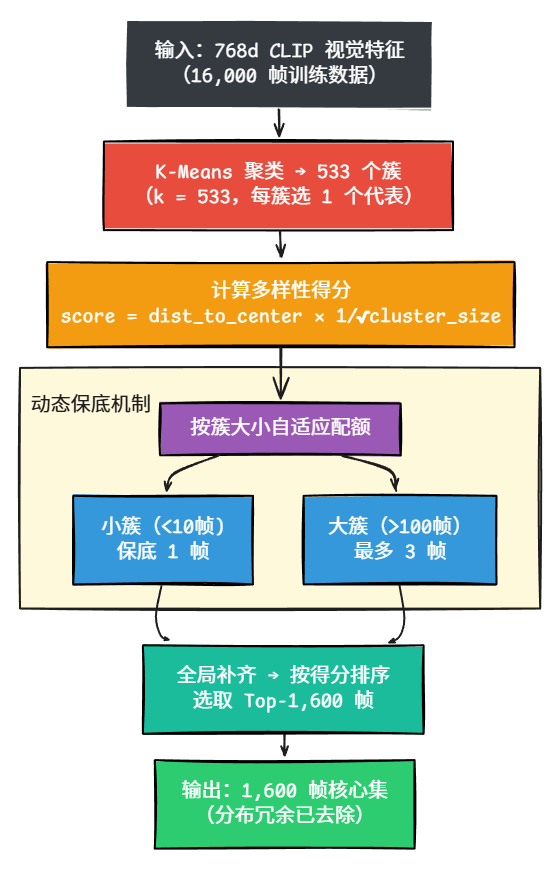
\includegraphics[width=0.45\textwidth]{figA_kmeans.png}
    \caption{自适应聚类筛选算法流程}
    \label{fig:kmeans_flow}
\end{figure}

\textbf{改进历程}（三次递进）：
\begin{itemize}[leftmargin=2em]
    \item \textbf{v1 固定保底}：每簇保底 1 帧 $\rightarrow$ 大簇（500 样本）严重浪费 $\rightarrow$ MSE = 0.004066；
    \item \textbf{v1.1 动态保底}：簇大小自适应配额（1--3 帧）$\rightarrow$ 更公平地挖掘内部多样性 $\rightarrow$ MSE = 0.003961；
    \item \textbf{v1.1 + PCA 400d 去噪}：PCA 降维后聚类 $\rightarrow$ \textbf{MSE = 0.003835}（全局第二）。
\end{itemize}

\textbf{实验结果}：自适应聚类筛选（v1.1 + PCA 400d）的 \textbf{Test MSE = 0.003835}，为全局第二。v1 固定保底（0.004066）因大簇浪费而表现平平，v1.1 动态保底（0.003961）通过公平配额小幅提升，PCA 400d 去噪（0.003835）是质变关键。核心结论：分布冗余定义有效，但需配合动态保底与 PCA 去噪才能释放潜力。

% -------------------- 3.2 时序冗余（事件分割）--------------------
\subsection{冗余定义二：时序冗余（事件分割视角）}
\label{sec:event_segmentation}

\textbf{核心假设}：动作变化率低的帧 = 时序冗余。大脑只保留打破预测的帧，过滤"发呆帧"。事件边界处分配更多记忆资源。

\textbf{脑机制映射}：海马体事件分割。人类会自动将连续行为切分为离散事件，事件边界（如"接近 $\rightarrow$ 抓取""抓取 $\rightarrow$ 转移"）处动作变化剧烈，应被优先保留。

\textbf{算法设计}（图~\ref{fig:temporal_boundary}）：将连续动作序列视为一个时序信号，通过检测"动作突变点"来识别事件边界。

\textbf{Step 1：动作变化率计算}。对每个 Episode 的 7DoF 动作序列 $a_t \in \mathbb{R}^7$，计算相邻帧的二范数变化率：
\begin{equation}
    \delta(t) = \|a_t - a_{t-1}\|_2
\end{equation}
$\delta(t)$ 度量了第 $t$ 帧相对于前一帧的动作剧烈程度。变化率低的帧对应平稳动作（如悬停等待），变化率高的帧对应动作转换（如"接近$\rightarrow$抓取"）。

\textbf{Step 2：事件边界识别}。设置百分位数阈值（90th percentile）作为硬阈值，所有 $\delta(t)$ 超过阈值的帧被视为候选边界。为避免噪声导致的虚假边界，进一步使用局部峰值检测：仅保留在 $\pm 3$ 帧邻域内为局部最大值的候选点。

\textbf{Step 3：边界保底与全局补齐}。识别出的事件边界帧自动进入核心集（保底机制）。若边界帧总数不足 1,600，则从非边界帧中按变化率降序补齐至目标大小；若超过 1,600，则按变化率截断至 Top-1,600。

\textbf{结果}：Test MSE = \textbf{0.008871}——\textbf{比随机基线（0.007229）还差 22.7\%}。

\textbf{失败原因分析}：单任务数据集（"接近 $\rightarrow$ 抓取 $\rightarrow$ 转移 $\rightarrow$ 放置"）时序耦合过强，50 个 Episode 的事件边界在视觉空间高度重叠。检测到的 539 个事件边界帧，本质上是 50 次重复的同一场景（图~\ref{fig:temporal_boundary}）。\textbf{核心教训}："时序分散"不等于"空间分散"，时序冗余定义与数据特性不匹配。

\begin{figure}[htbp]
    \centering
    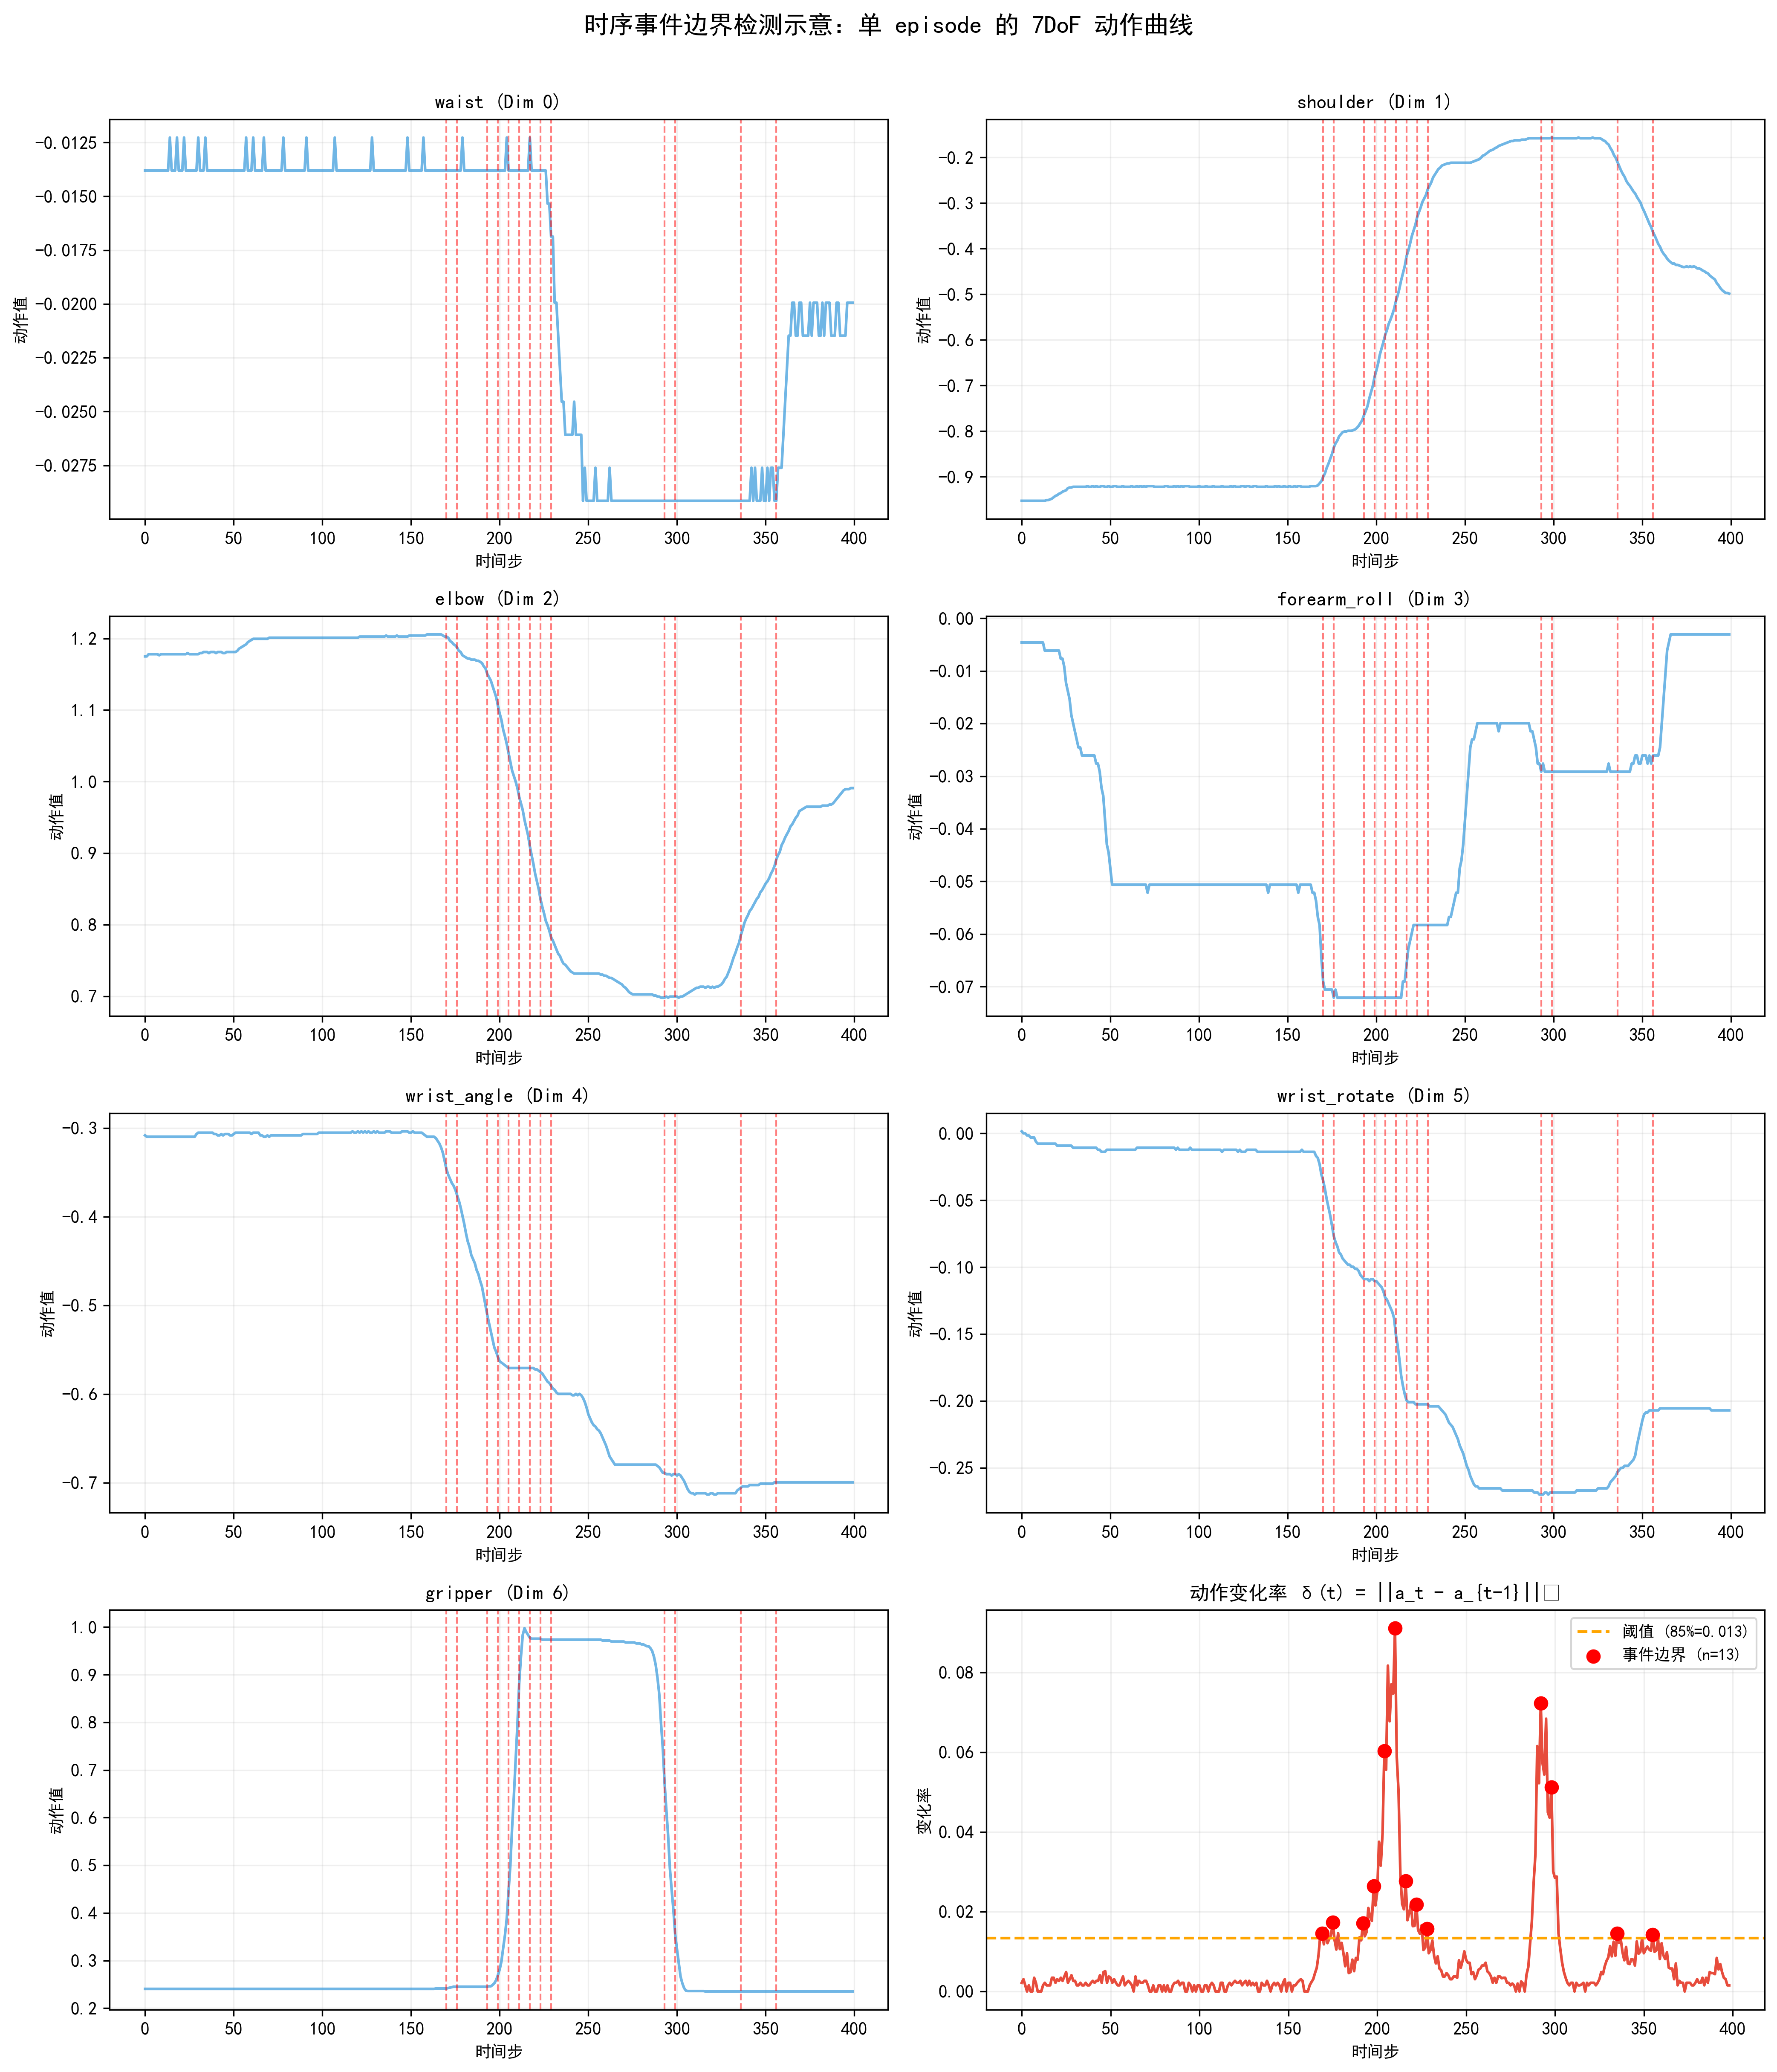
\includegraphics[width=0.95\textwidth]{fig12_temporal_boundary}
    \caption{时序事件边界检测结果。边界帧在特征空间高度重叠}
    \label{fig:temporal_boundary}
\end{figure}

% -------------------- 3.3 预测编码 --------------------
\subsection{冗余定义三：时序冗余（预测编码视角）}
\label{sec:predictive}

\textbf{核心假设}：用历史动作能准确预测的当前帧 = 时序冗余。大脑本质上是一个预测机器，预测误差小的帧对应神经元"低更新状态"，在训练数据中即为冗余。

\textbf{脑机制映射}：预测编码（Predictive Coding）。根据 Millidge et al. (2021)，大脑持续生成下一时刻的感官预测，当实际输入与预测一致时，神经活动被抑制；仅当预测误差超过阈值时，信息才被向上传递\cite{millidge2021predictive}。

% ===== 图C：预测编码滑动窗口流程 =====

\textbf{算法设计}（图~\ref{fig:predictive_coding_flow}）：核心思想是"可预测 = 冗余"——如果一个帧的动作可以被历史动作准确预测，则该帧包含的新信息极少。

\textbf{Step 1：滑动窗口构建}。对每个 Episode 内的帧 $t$，取历史 5 帧动作向量 $[a_{t-5}, \dots, a_{t-1}]$ 作为输入特征。前 5 帧无法用完整窗口时，用一阶差分外推填充。

\textbf{Step 2：最小二乘线性回归}。在每个 Episode 内独立训练线性模型：
\begin{equation}
    \hat{a}_t = W \cdot [a_{t-5}, \dots, a_{t-1}] + b, \quad r_t = \|a_t - \hat{a}_t\|_2
\end{equation}
其中 $W \in \mathbb{R}^{7 \times 35}$，$b \in \mathbb{R}^7$。通过最小二乘法求解：$W, b = \arg\min \sum_{t} \|a_t - \hat{a}_t\|^2_2$。每个 Episode 独立建模的原因是不同 Episode 的动作模式存在系统性差异（起始位置、速度不同），全局模型会引入偏差。

\textbf{Step 3：残差计算与排序}。残差小的帧 = 可预测 = 时序冗余；残差大的帧 = 打破预测 = 高价值。全局按残差降序取 Top-1,600 帧。

\begin{figure}[H]
    \centering
    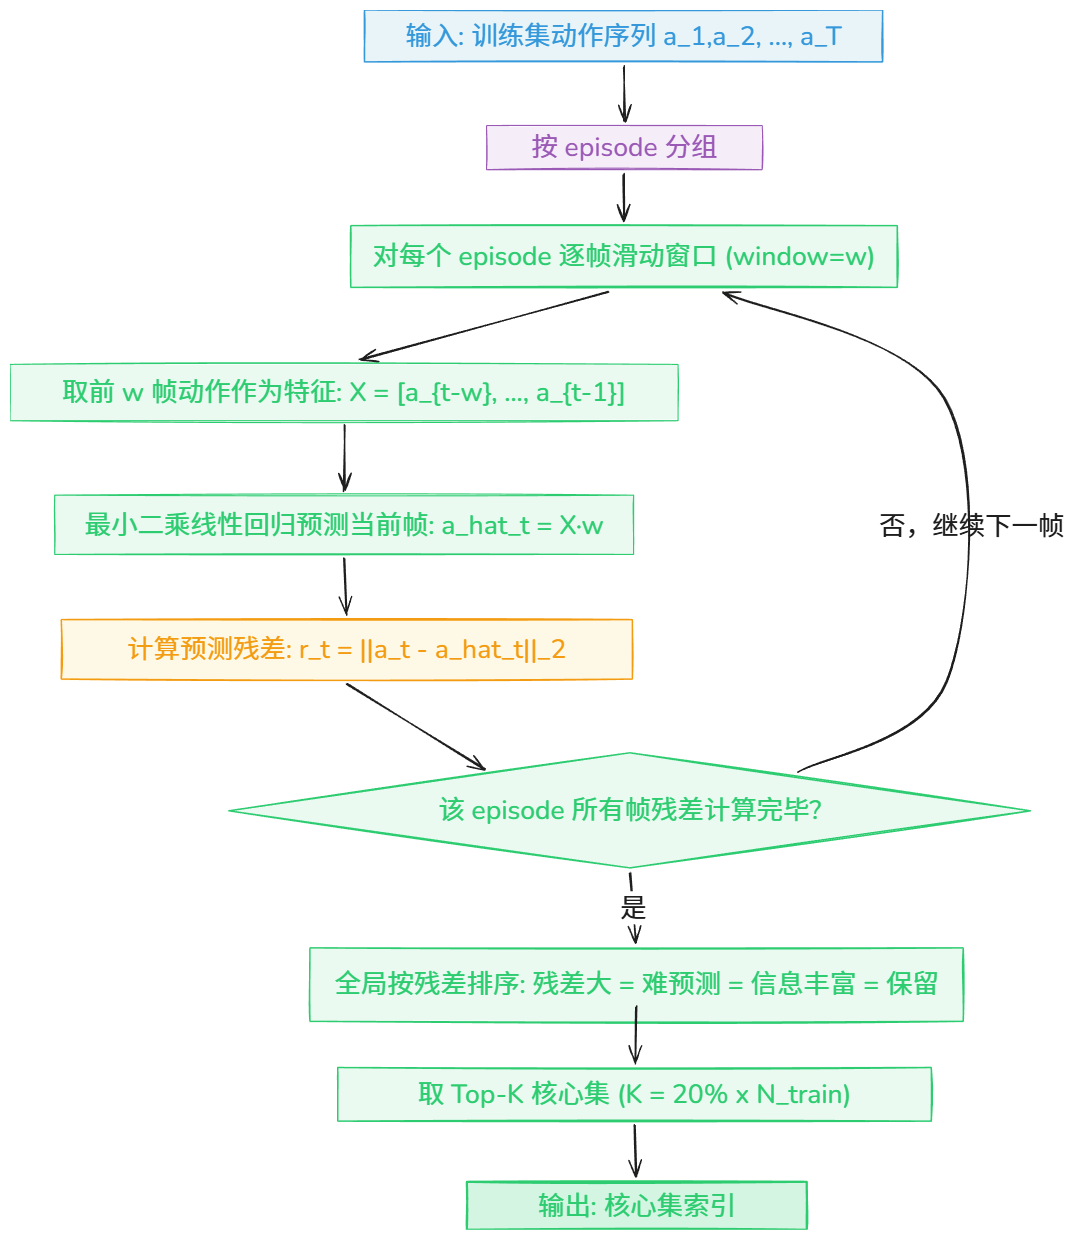
\includegraphics[width=0.70\textwidth]{figC_predictive_coding.png}
    \caption{预测编码滑动窗口流程}
    \label{fig:predictive_coding_flow}
\end{figure}

\textbf{结果}：单尺度 window=5 的 Test MSE = \textbf{0.005688}，较随机基线降低 21.3\%。

\textbf{成功之处}：滑动窗口自回归预测确实能区分时序冗余帧（残差小）和高价值帧（残差大），证明了"可预测性 = 冗余"这一假设的合理性。与事件分割（动作变化率差分，MSE 0.008871）相比，利用 window=5 的历史上下文建模了动作的时序依赖关系，显著优于仅利用相邻帧一阶信息的差分方法。

\textbf{局限与改进尝试}：
\begin{itemize}[leftmargin=2em]
    \item \textbf{单尺度最优}：window=5 的 Test MSE = 0.005688，是 window$\in\{3,5,10,15\}$ 中的最优值；
    \item \textbf{多尺度融合失败}：window=3, 5, 10 的残差范围差异 100 倍，直接融合导致量纲灾难（MSE 0.007194）；归一化后融合（MSE 0.006734）因信号高度相关而无信息增益；
    \item \textbf{联合得分失败}：预测误差 $\times$ 动作变化率联合（MSE 0.005963），因变化率主导融合结果而劣于单尺度。
\end{itemize}

\textbf{核心教训}：在这个单任务数据集上，时序模式非常规律，线性回归在 5 帧窗口内已能提取几乎全部可用信息。增加尺度数量或联合其他信号并不能带来信息增益——冗余信号必须是正交互补的，高度相关的信号融合只会放大噪声。

% -------------------- 3.4 压缩冗余 --------------------
\subsection{冗余定义四：压缩冗余（自编码器视角）}
\label{sec:ae}

\textbf{核心假设}：重建误差小的帧 = 模型已学会 = 压缩冗余。对"看不懂"的帧（重建误差大）分配更多注意力。

\textbf{脑机制映射}：意外检测机制。大脑对无法内化的刺激保持敏感，自编码器重建误差正是这一机制的量化实现。

\textbf{算法设计}（图~\ref{fig:ae_reconstruction}）：自编码器（Autoencoder, AE）通过重构输入特征来检测"意外"——重构误差大的帧对应模型无法内化的模式，应被优先保留。

\textbf{网络结构}。输入 768d CLIP 视觉特征 $f \in \mathbb{R}^{768}$。Encoder 为对称压缩结构：
\begin{itemize}[leftmargin=2em]
    \item FC-1：$768 \rightarrow 512$，ReLU 激活
    \item FC-2：$512 \rightarrow 256$，ReLU 激活
    \item Bottleneck：$256 \rightarrow h$，无激活（$h \in \{128, 64, 32\}$ 为三种压缩配置）
\end{itemize}
Decoder 为对称解压结构，Bottleneck $\rightarrow 256 \rightarrow 512 \rightarrow 768$，中间层 ReLU 激活，输出层线性激活。重建目标为最小化均方误差：
\begin{equation}
    \mathcal{L} = \frac{1}{N} \sum_{i=1}^{N} \|f_i - \hat{f}_i\|^2_2
\end{equation}

\textbf{训练配置}。在全部 16,000 帧上训练，优化器 Adam（lr=1e-3），Batch Size=256，训练 200 epochs 或验证 Loss 连续 20 epoch 不下降则早停。

\textbf{核心集选择}。训练完成后，计算每帧的重建误差 $e_i = \|f_i - \hat{f}_i\|^2_2$。重建误差小的帧被视为"已学会"（压缩冗余），重建误差大的帧被视为"意外"而保留。按重建误差降序选取 Top-1,600 帧。

\textbf{结果}：三种配置均失败（表~\ref{tab:ae_results}）。

\begin{table}[htbp]
\centering
\caption{自编码器不同压缩比的实验结果}
\label{tab:ae_results}
\begin{tabular}{@{}cccc@{}}
\toprule
\textbf{隐藏层} & \textbf{压缩比} & \textbf{Test MSE} & \textbf{状态} \\
\midrule
128d & 6:1 & 0.007292 & 失败 \\
64d & 12:1 & 0.007019 & 边际 \\
32d & 24:1 & 0.008290 & 失败 \\
\bottomrule
\end{tabular}
\end{table}

\textbf{失败原因分析}：CLIP 特征本身高度规整（预训练压缩后的抽象表示），数据集视觉变化范围有限（同一任务、同一场景、同一物体）。AE 训练 Loss 极低（$10^{-6}$ 量级），重建误差区分度几乎为零。\textbf{核心教训}：在已高度压缩的特征上再做压缩，无法获得有效信号。

\begin{figure}[htbp]
    \centering
    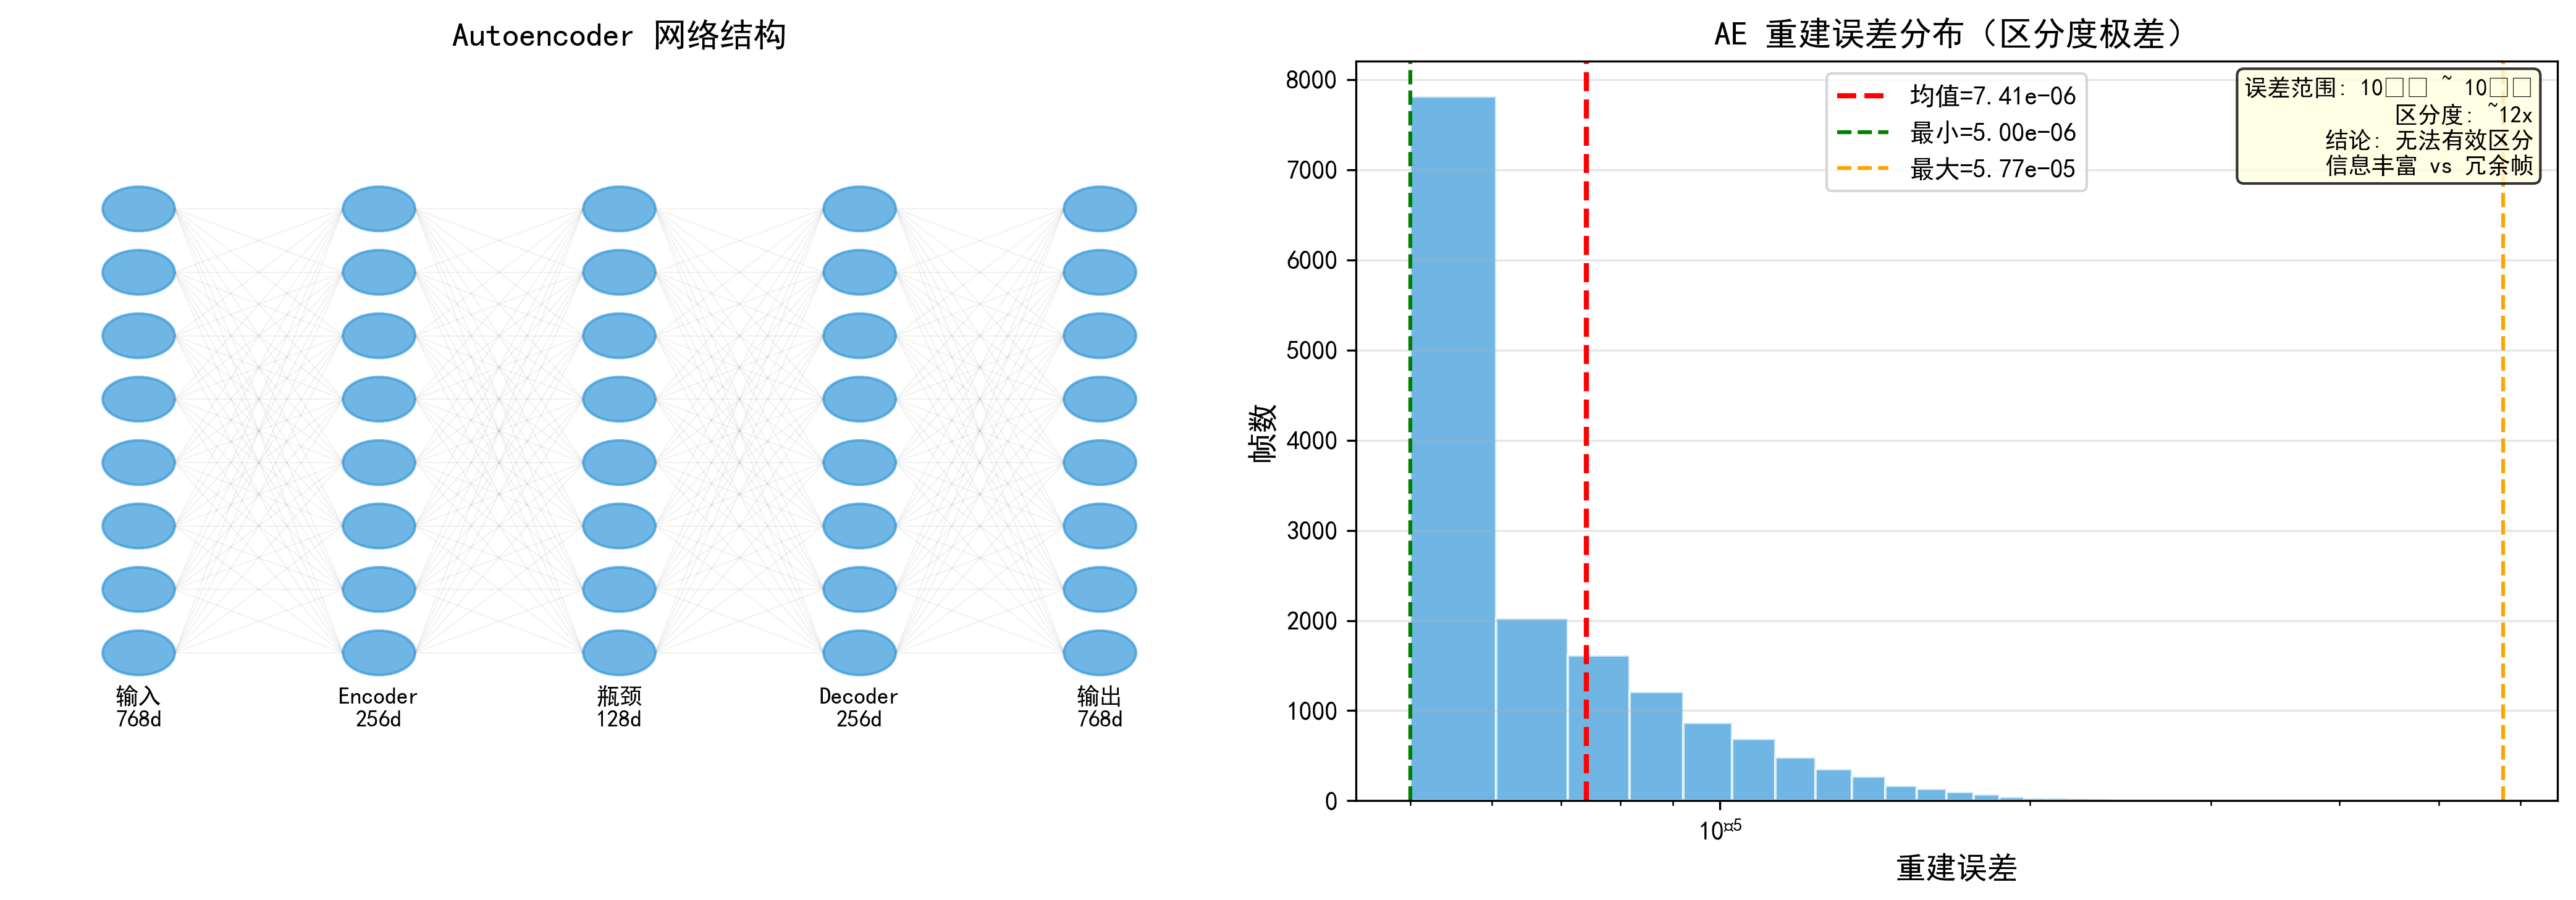
\includegraphics[width=0.95\textwidth]{fig13_ae_reconstruction}
    \caption{自编码器重建网络结构；重建误差分布}
    \label{fig:ae_reconstruction}
\end{figure}

% -------------------- 3.5 几何覆盖冗余 --------------------
\subsection{冗余定义五：几何覆盖冗余（FPS + 密度过滤视角）}
\label{sec:fps}

\textbf{核心假设}："最远"不等于"最好"，但"远且不孤立"等于"最好"。空间覆盖是核心价值，但需要剔除边缘噪声。

\textbf{脑机制映射}：海马体空间编码 $\rightarrow$ 几何覆盖。海马体中的 place cell 通过几何位置关系编码空间信息，对应特征空间中的最远点采样（Farthest Point Sampling, FPS）——优先选择距离已选集合最远的点，以保证空间覆盖的完整性。

% ===== 图B：密度过滤FPS流程 =====

\textbf{算法设计}（图~\ref{fig:fps_flow}）：核心思想是"远且不孤立 = 最好"。标准 FPS 保证空间覆盖，但会选到边缘噪声；密度过滤温和修正这一缺陷。

\textbf{Step 1：标准 FPS 候选集}。输入 768d 视觉特征（16,000 帧）。贪心策略迭代选择最远点：初始随机选 1 帧，每次选择距离已选集合最远的帧，直至选出 1,600 帧候选核心集。

\textbf{Step 2：k-NN 局部密度估计}。对候选集中的每帧，在全部 16,000 帧中找 $k=6$ 个最近邻（欧氏距离），计算平均邻域距离作为局部密度度量。密度越高 = 邻域越密集 = 越典型；密度越低 = 越孤立 = 越可能是噪声。

\textbf{Step 3：密度过滤替换}。将候选集中 15\%（240 帧）局部密度最低的点识别为"疑似噪声"。对每个被替换点，在全局未选帧中寻找局部密度最高的帧作为替换候选。

\textbf{Step 4：输出}。输出"远且不孤立"的 1,600 帧核心集。

\begin{figure}[H]
    \centering
    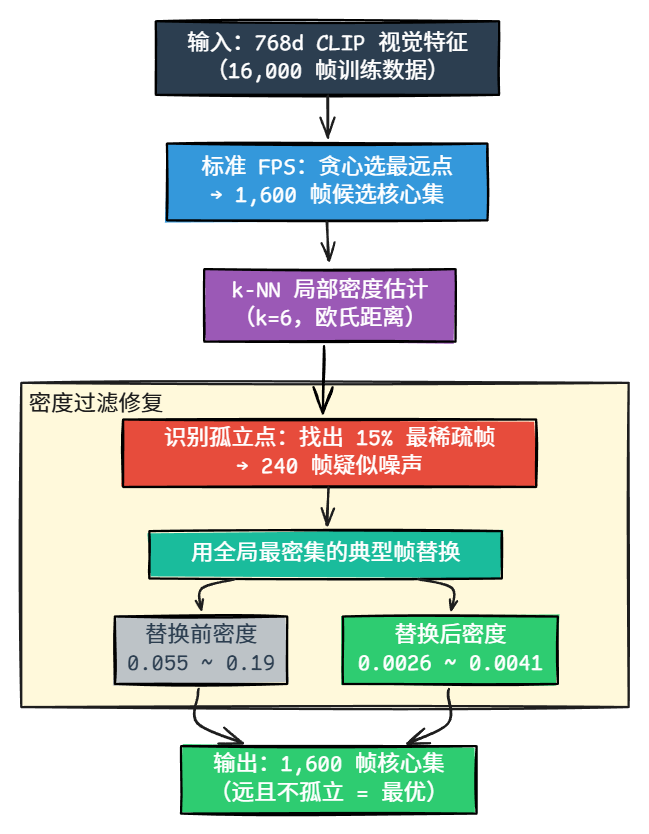
\includegraphics[width=0.45\textwidth]{figB_fps.png}
    \caption{密度过滤 FPS 算法流程}
    \label{fig:fps_flow}
\end{figure}

\textbf{改进历程}：
\begin{itemize}[leftmargin=2em]
    \item \textbf{标准 FPS}：MSE = 0.004294，但选到极端离群噪声点；
    \item \textbf{加权 FPS（3 种策略均失败）}：feature\_norm 权重（CLIP 已 L2 归一化，无区分度）、action\_delta 权重（时序变化率与空间位置不正交）、local\_density 权重（过度强化稀疏偏好，选到极端噪声）；
    \item \textbf{密度过滤 FPS}：\textbf{MSE = 0.003792}（全局最优）。
\end{itemize}

\textbf{实验结果}：密度过滤 FPS 的 \textbf{Test MSE = 0.003792}，为全局最优。标准 FPS（0.004294）因边缘噪声点拖累，加权 FPS 三种策略均失败。核心结论："最远"不等于"最好"，但"远且不孤立"等于"最好"。

% -------------------- 3.6 五种冗余定义对比 --------------------
\subsection{从失败中学习：五种冗余定义的对比总结}
\label{sec:comparison}

前五节的探索呈现了一条清晰的"试错—修正"曲线。分布冗余（K-Means 视角）的成功验证了"特征空间过度聚集 = 冗余"这一假设的合理性，但它的成功并非一帆风顺：固定保底机制下大簇严重浪费名额，自适应配额后才趋于公平，PCA 400d 去噪后才达到精度顶峰。事件分割（动作变化率检测）的失败揭示了一个关键事实：单任务数据集的时序结构高度重复，"事件边界"在特征空间中并不提供新的信息。压缩冗余的失败则说明，在已经高度压缩的 CLIP 特征上再做压缩，信号已经被预训练模型榨干，AE 无法区分信息的"难易程度"。几何覆盖冗余的成功是最意外的：它放弃了 K-Means 的"簇"这一中间抽象，直接在原始特征空间优化最大最小距离覆盖，同时用 k-NN 局部密度修复 FPS 的离群倾向。预测编码滑动窗口的成功（MSE 0.005688）证明了"可预测性 = 冗余"的理论假设，但受限于单任务数据集的动作规律性和线性模型的表达能力，未能达到几何覆盖冗余的精度水平。这条路径告诉我们：有时候更直接的优化目标反而更有效。

\begin{table}[htbp]
\centering
\caption{五种冗余定义的综合对比}
\label{tab:redundancy_comparison}
\begin{tabular}{@{}lclcc@{}}
\toprule
\textbf{冗余定义} & \textbf{核心假设} & \textbf{匹配度} & \textbf{最佳 MSE} & \textbf{结论} \\
\midrule
分布冗余 & 特征空间过度聚集 = 冗余 & 高 & 0.003835 & 成功 \\
事件分割 & 动作变化率低 = 冗余 & 低 & 0.008871 & 失败 \\
预测编码 & 可预测 = 冗余 & 中 & 0.005688 & 有效但有限 \\
压缩冗余 & 重建误差小 = 已学会 & 极低 & $\sim$0.007 & 失败 \\
几何覆盖冗余 & 远且不孤立 = 最好 & \textbf{最高} & \textbf{0.003792} & \textbf{最优} \\
\bottomrule
\end{tabular}
\end{table}

\textbf{独立思考的核心结论}："冗余"的定义不是普适的，必须与\textbf{数据特性}（单任务/多任务、原始像素/预训练特征）和\textbf{目标任务}（动作预测/分类/生成）高度匹配。本文的否定性验证（时序、AE、多种融合均失败）恰恰证明了这一点。

\begin{figure}[htbp]
    \centering
    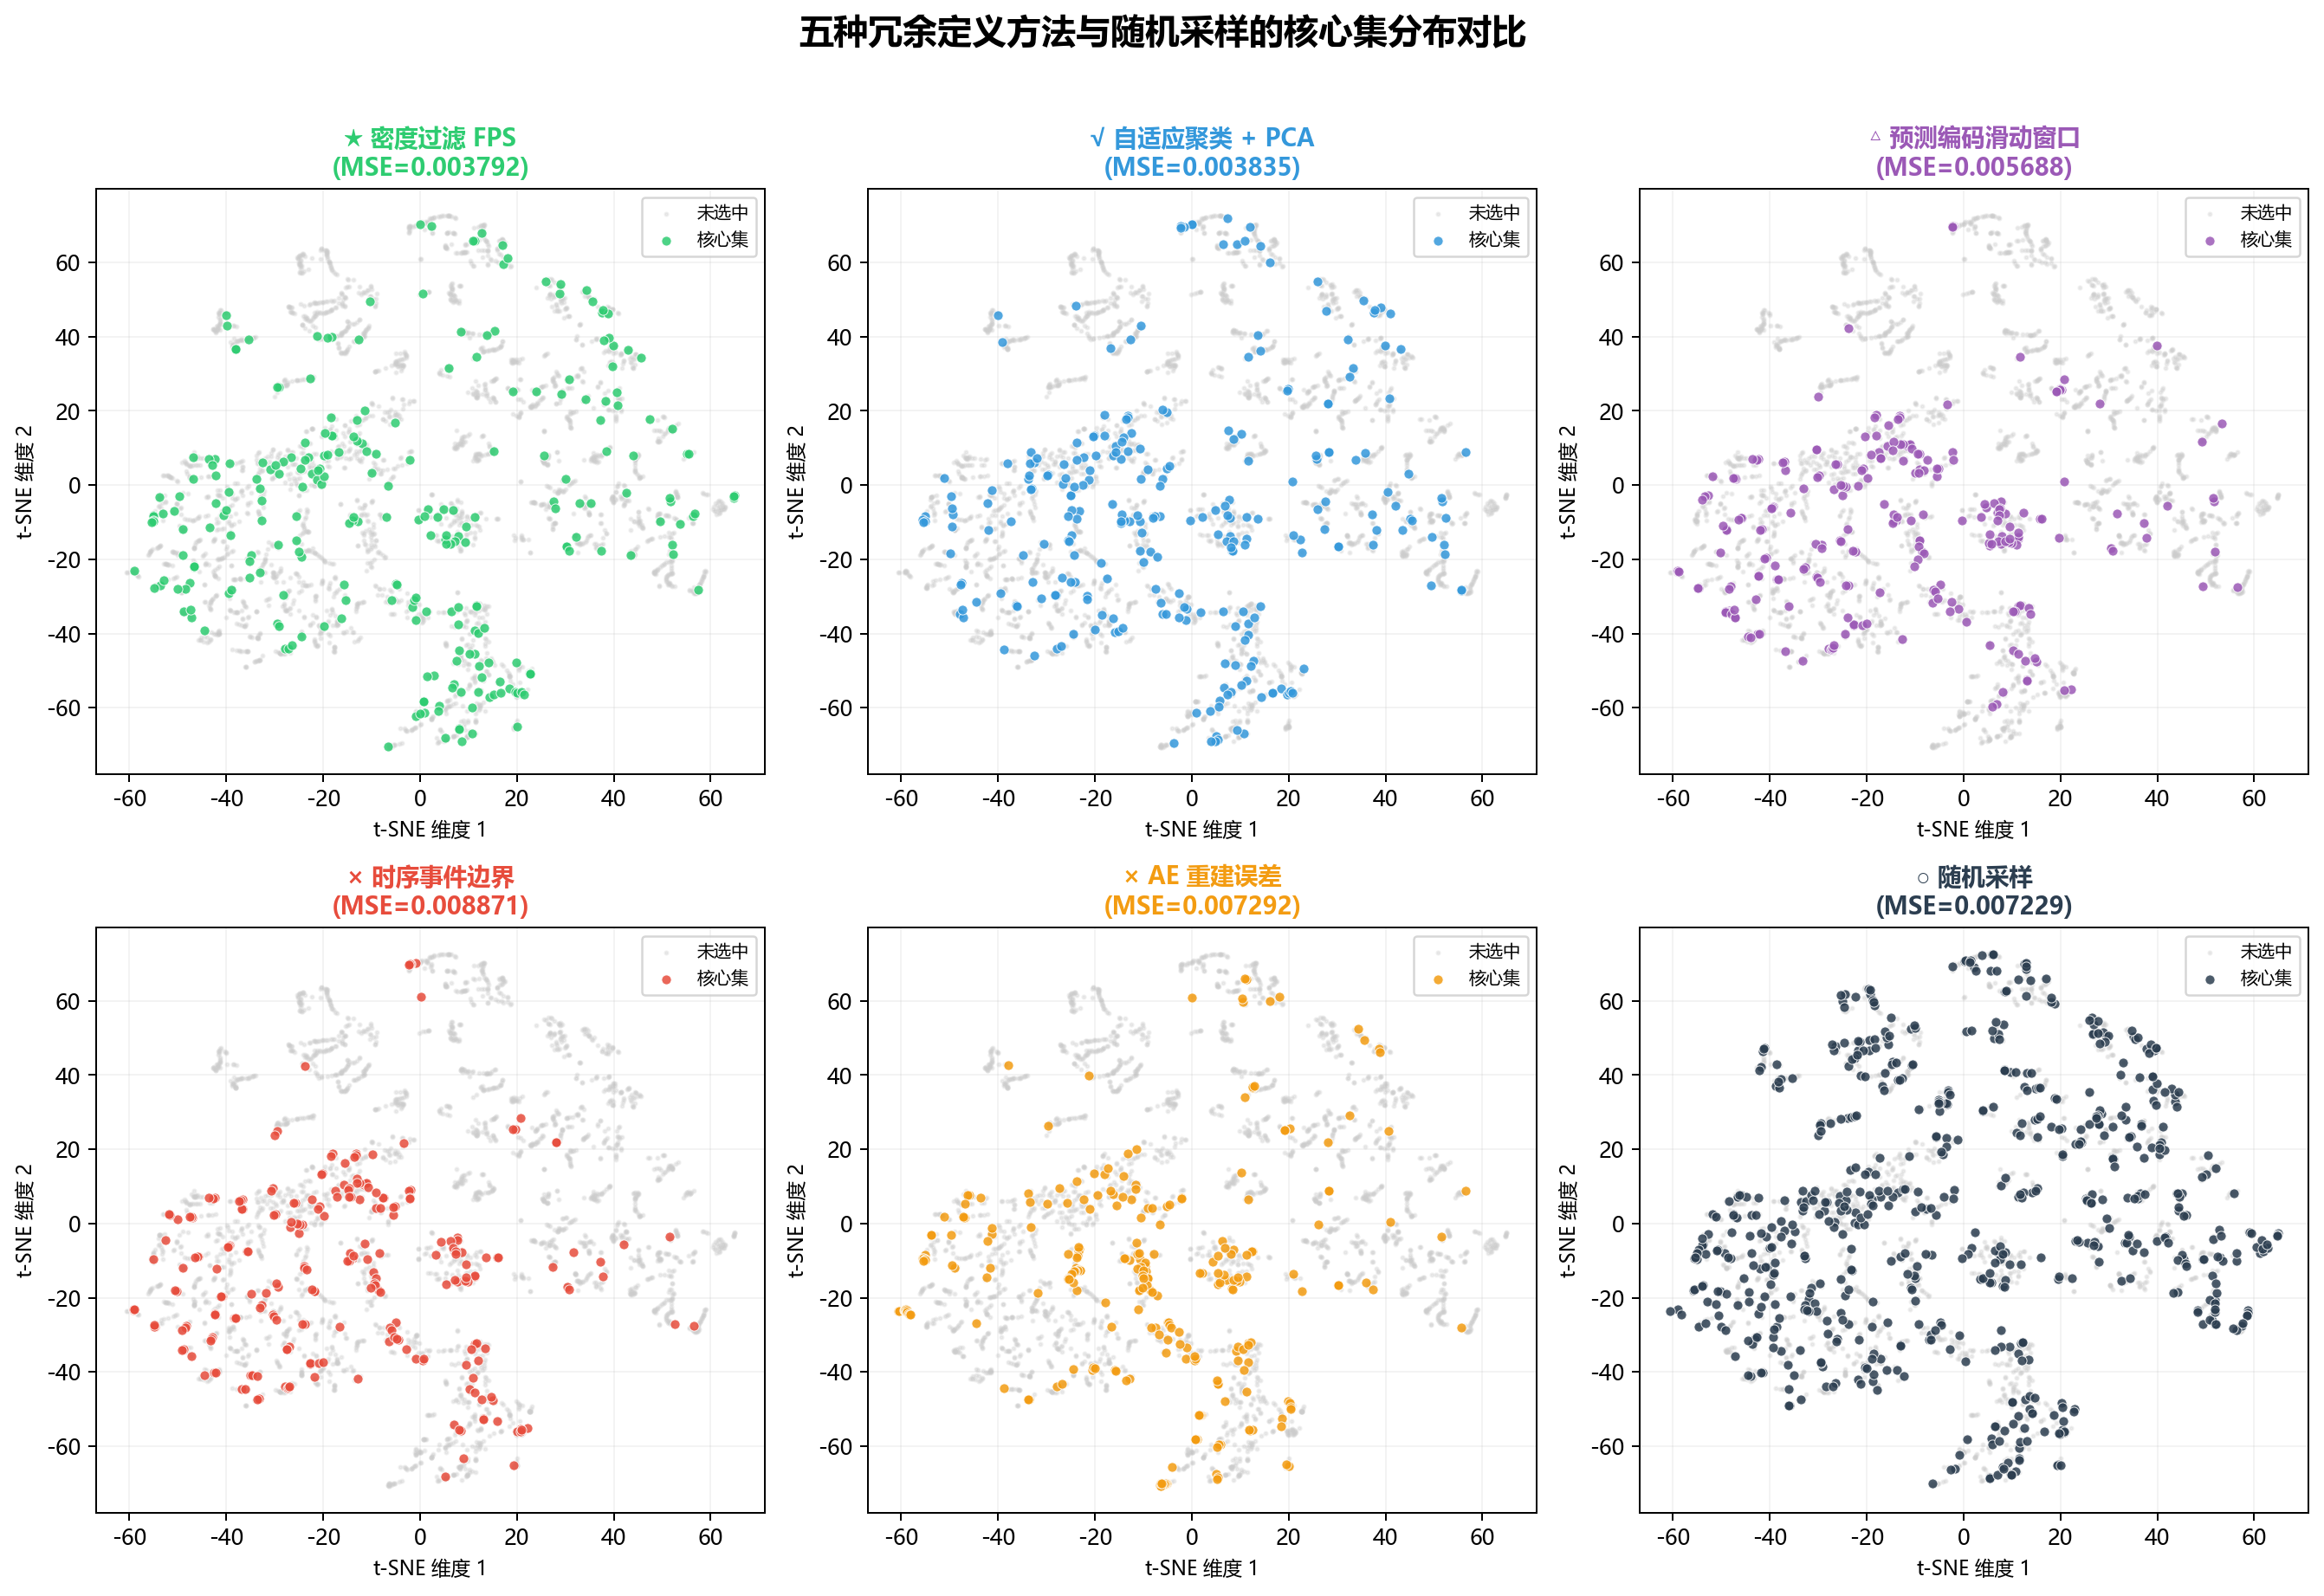
\includegraphics[width=0.95\textwidth]{fig11_redundancy_comparison}
    \caption{五种冗余定义选择结果的 t-SNE 可视化对比（2$\times$3 网格）}
    \label{fig:redundancy_comparison}
\end{figure}

图~\ref{fig:redundancy_comparison}的 t-SNE 可视化直观展示了五种方法的差异：密度过滤 FPS（左上）覆盖最均匀；自适应聚类筛选（中上）次之；预测编码（右上）在某些区域有聚集；时序边界（左下）高度聚集；AE 重建误差（中下）分布随机；随机采样（右下）聚集于高密度区域。


% ==================== 4. 成功思路深入分析 ====================
\section{成功思路的深入分析}
\label{sec:success}

\subsection{K-Means 系列：从固定保底到 PCA 去噪}

\subsubsection{动态保底的价值}

固定保底聚类筛选中，533 个簇无论大小都保底 1 帧。大簇（500 样本）只选 1 帧 $\rightarrow$ 严重浪费，500 个样本的多样性只被 1 帧代表。自适应聚类筛选让大簇最多 3 帧（$\text{quota} = \max(1, \min(3, \lfloor \text{size}/50 \rfloor + 1))$），更公平地挖掘内部多样性。改进幅度有限（2.6\%），但工程价值高：选择更"公平"，大簇不再被严重低估。

\subsubsection{PCA 400d 的反直觉发现}

400d（保留 99.8\% 方差）比 768d 原始特征效果更好。原因：去掉的 0.2\% 方差（约 368 维）是干扰 K-Means 聚类的噪声方向。600d 悖论：保留 100\% 方差但效果更差 $\rightarrow$ PCA 线性变换本身在大于 400d 时引入有害变换。这一发现强调了"恰到好处的简化"的价值——不是所有信息都有助于聚类，噪声方向会干扰簇边界的判定（图~\ref{fig:pca_sweep}）。

\begin{figure}[htbp]
    \centering
    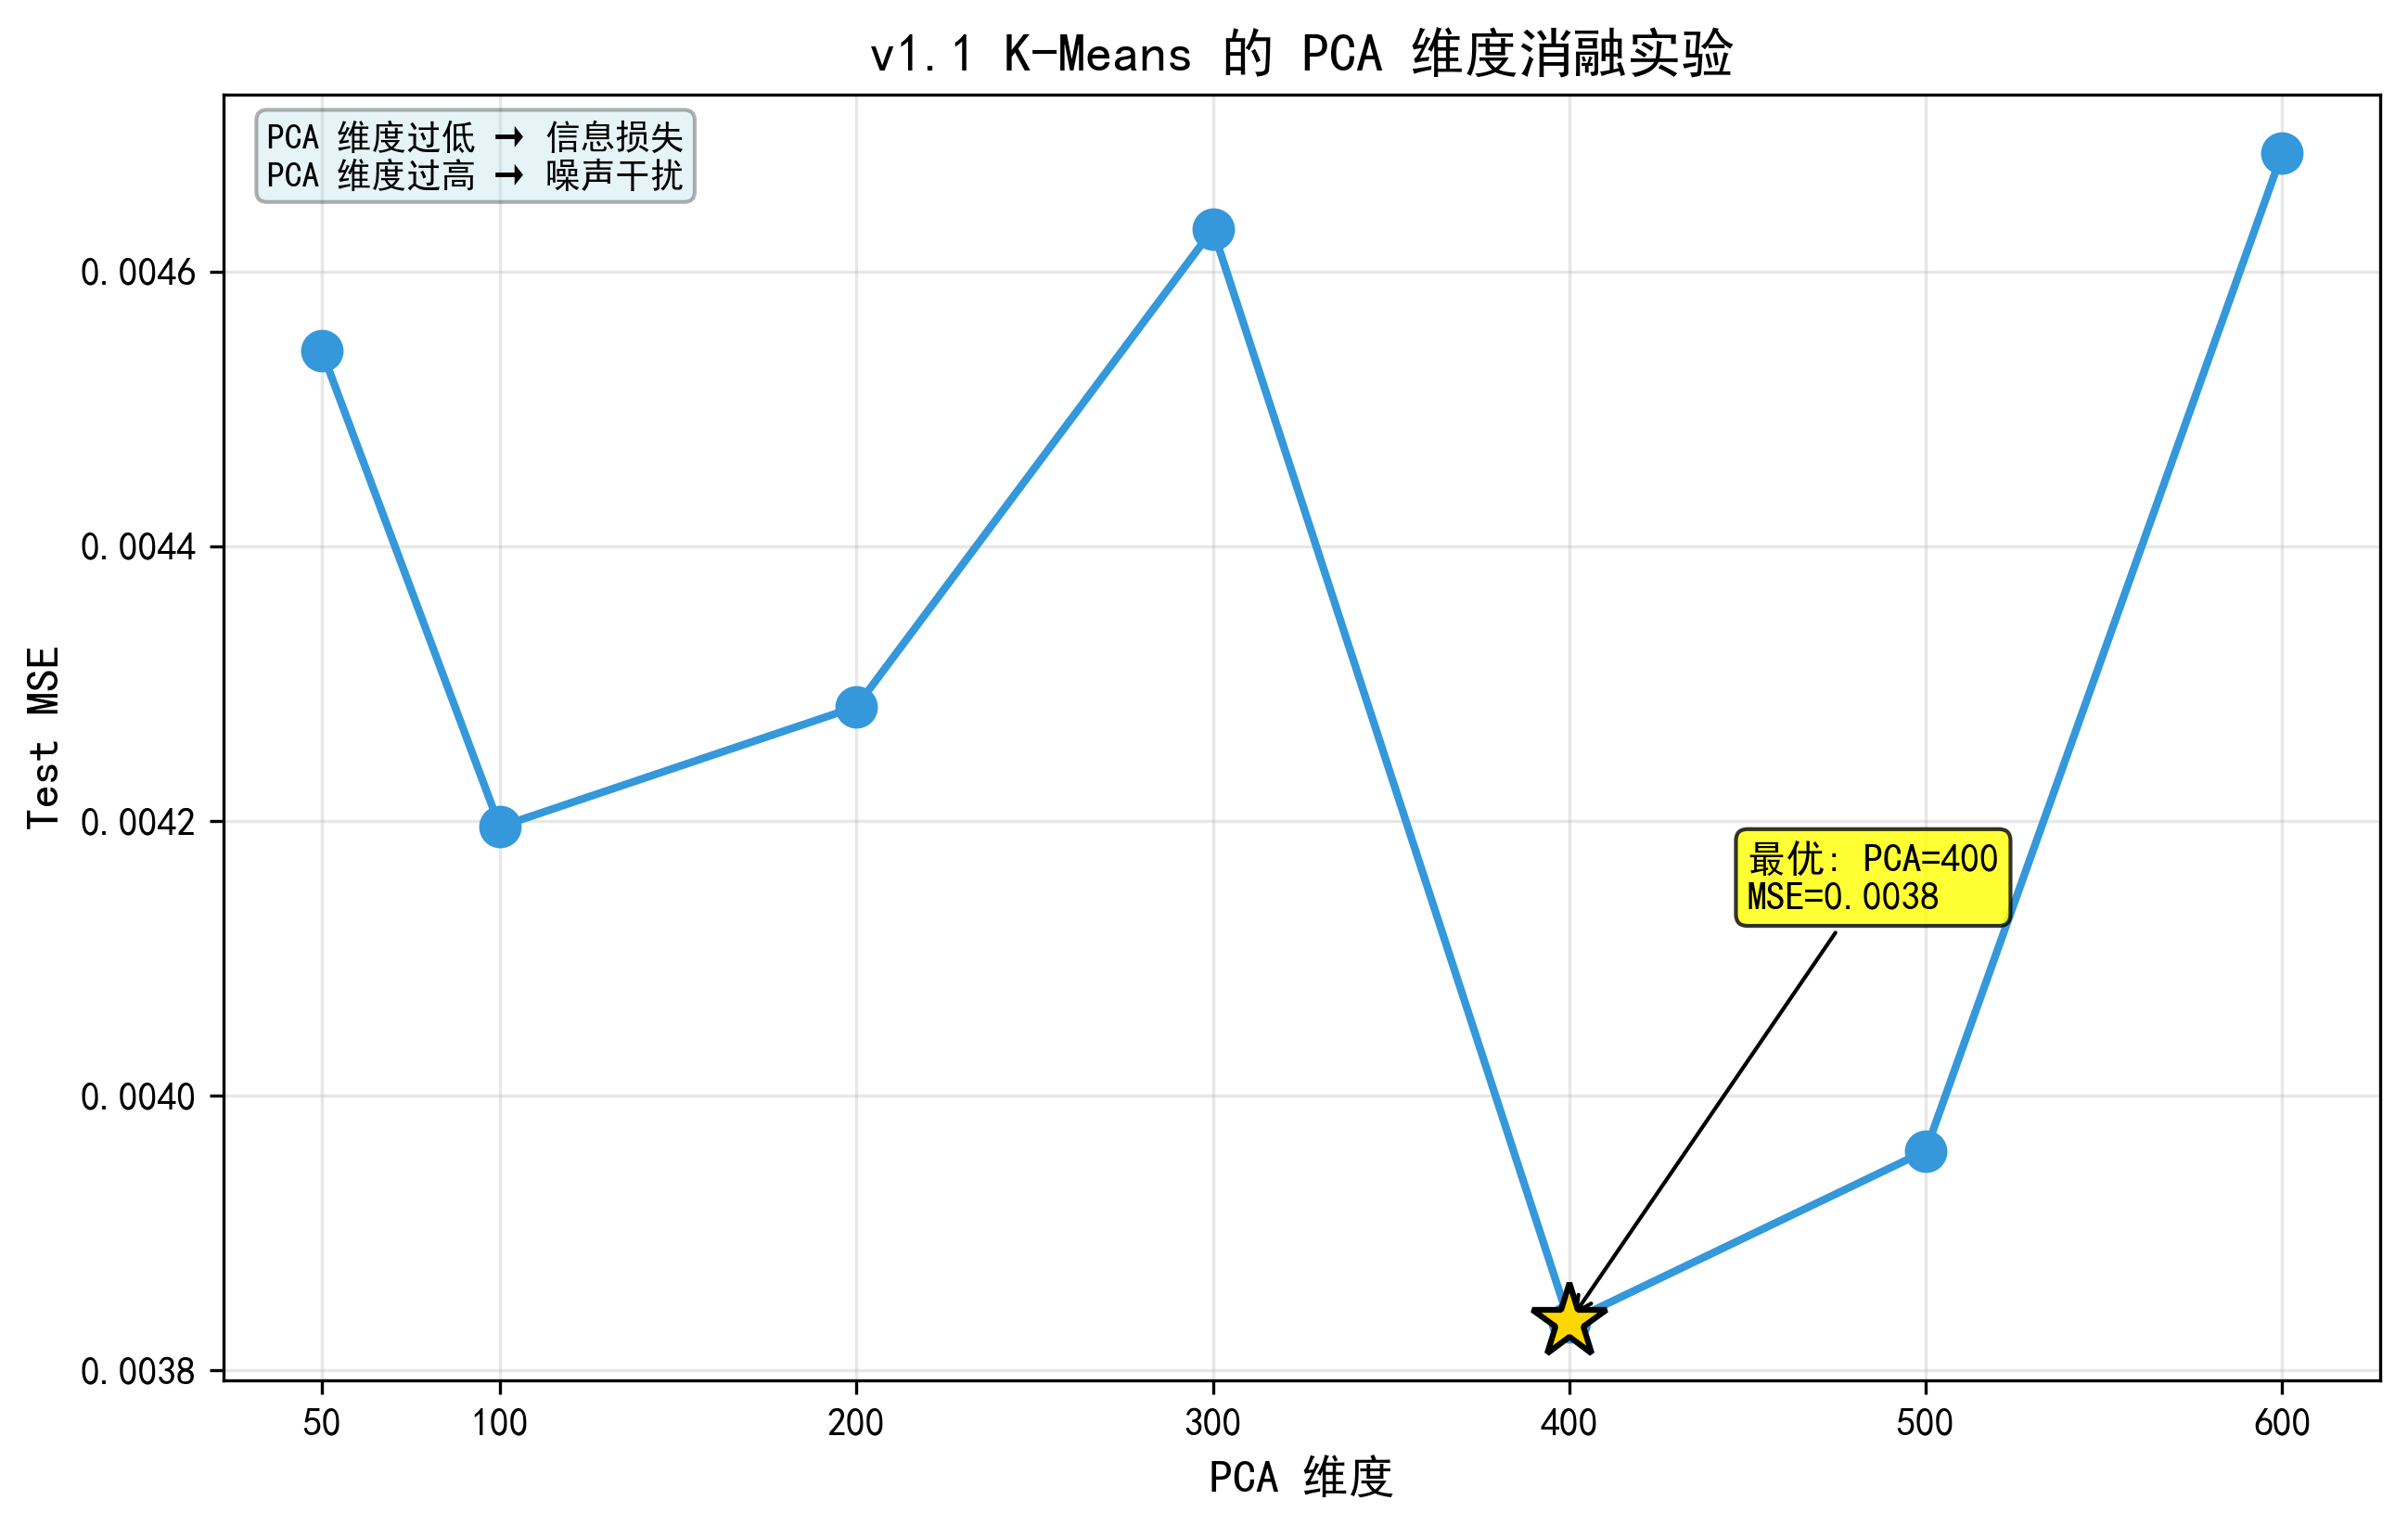
\includegraphics[width=0.75\textwidth]{fig9_pca_sweep}
    \caption{PCA 维度消融曲线。400d 为 sweet spot，600d 反而更差}
    \label{fig:pca_sweep}
\end{figure}

\subsection{FPS 系列：从标准覆盖到密度过滤}

\subsubsection{标准 FPS 的盲区}

贪心策略在特征空间"边缘"选点，这些边缘点可能是传感器噪声或极端姿态，教学价值为零。标准 FPS 的 Test MSE = 0.004294，已优于随机基线，但离最优仍有差距。

\subsubsection{密度过滤的修复机制}

标准 FPS 选出的 1,600 帧中，240 帧（15\%）被识别为极端稀疏孤立点。替换为全局高密度典型帧后，新帧密度：0.0026--0.0041（原：0.055--0.19）。覆盖保证 + 质量过滤 = 最优结果。密度过滤的精妙之处在于"温和修正"：只替换最边缘的 15\%，保留 FPS 的核心覆盖能力（图~\ref{fig:density_replacement}）。

图~\ref{fig:tsne}的 t-SNE 可视化进一步展示了密度过滤 FPS 的空间覆盖优势：红色核心集在二维投影中均匀分布，而蓝色随机采样大量聚集于高密度区域，边缘稀疏区几乎空白。这说明 FPS 机制确实选到了"代表性"帧，而随机采样遗漏了关键边缘信息。

\begin{figure}[H]
    \centering
    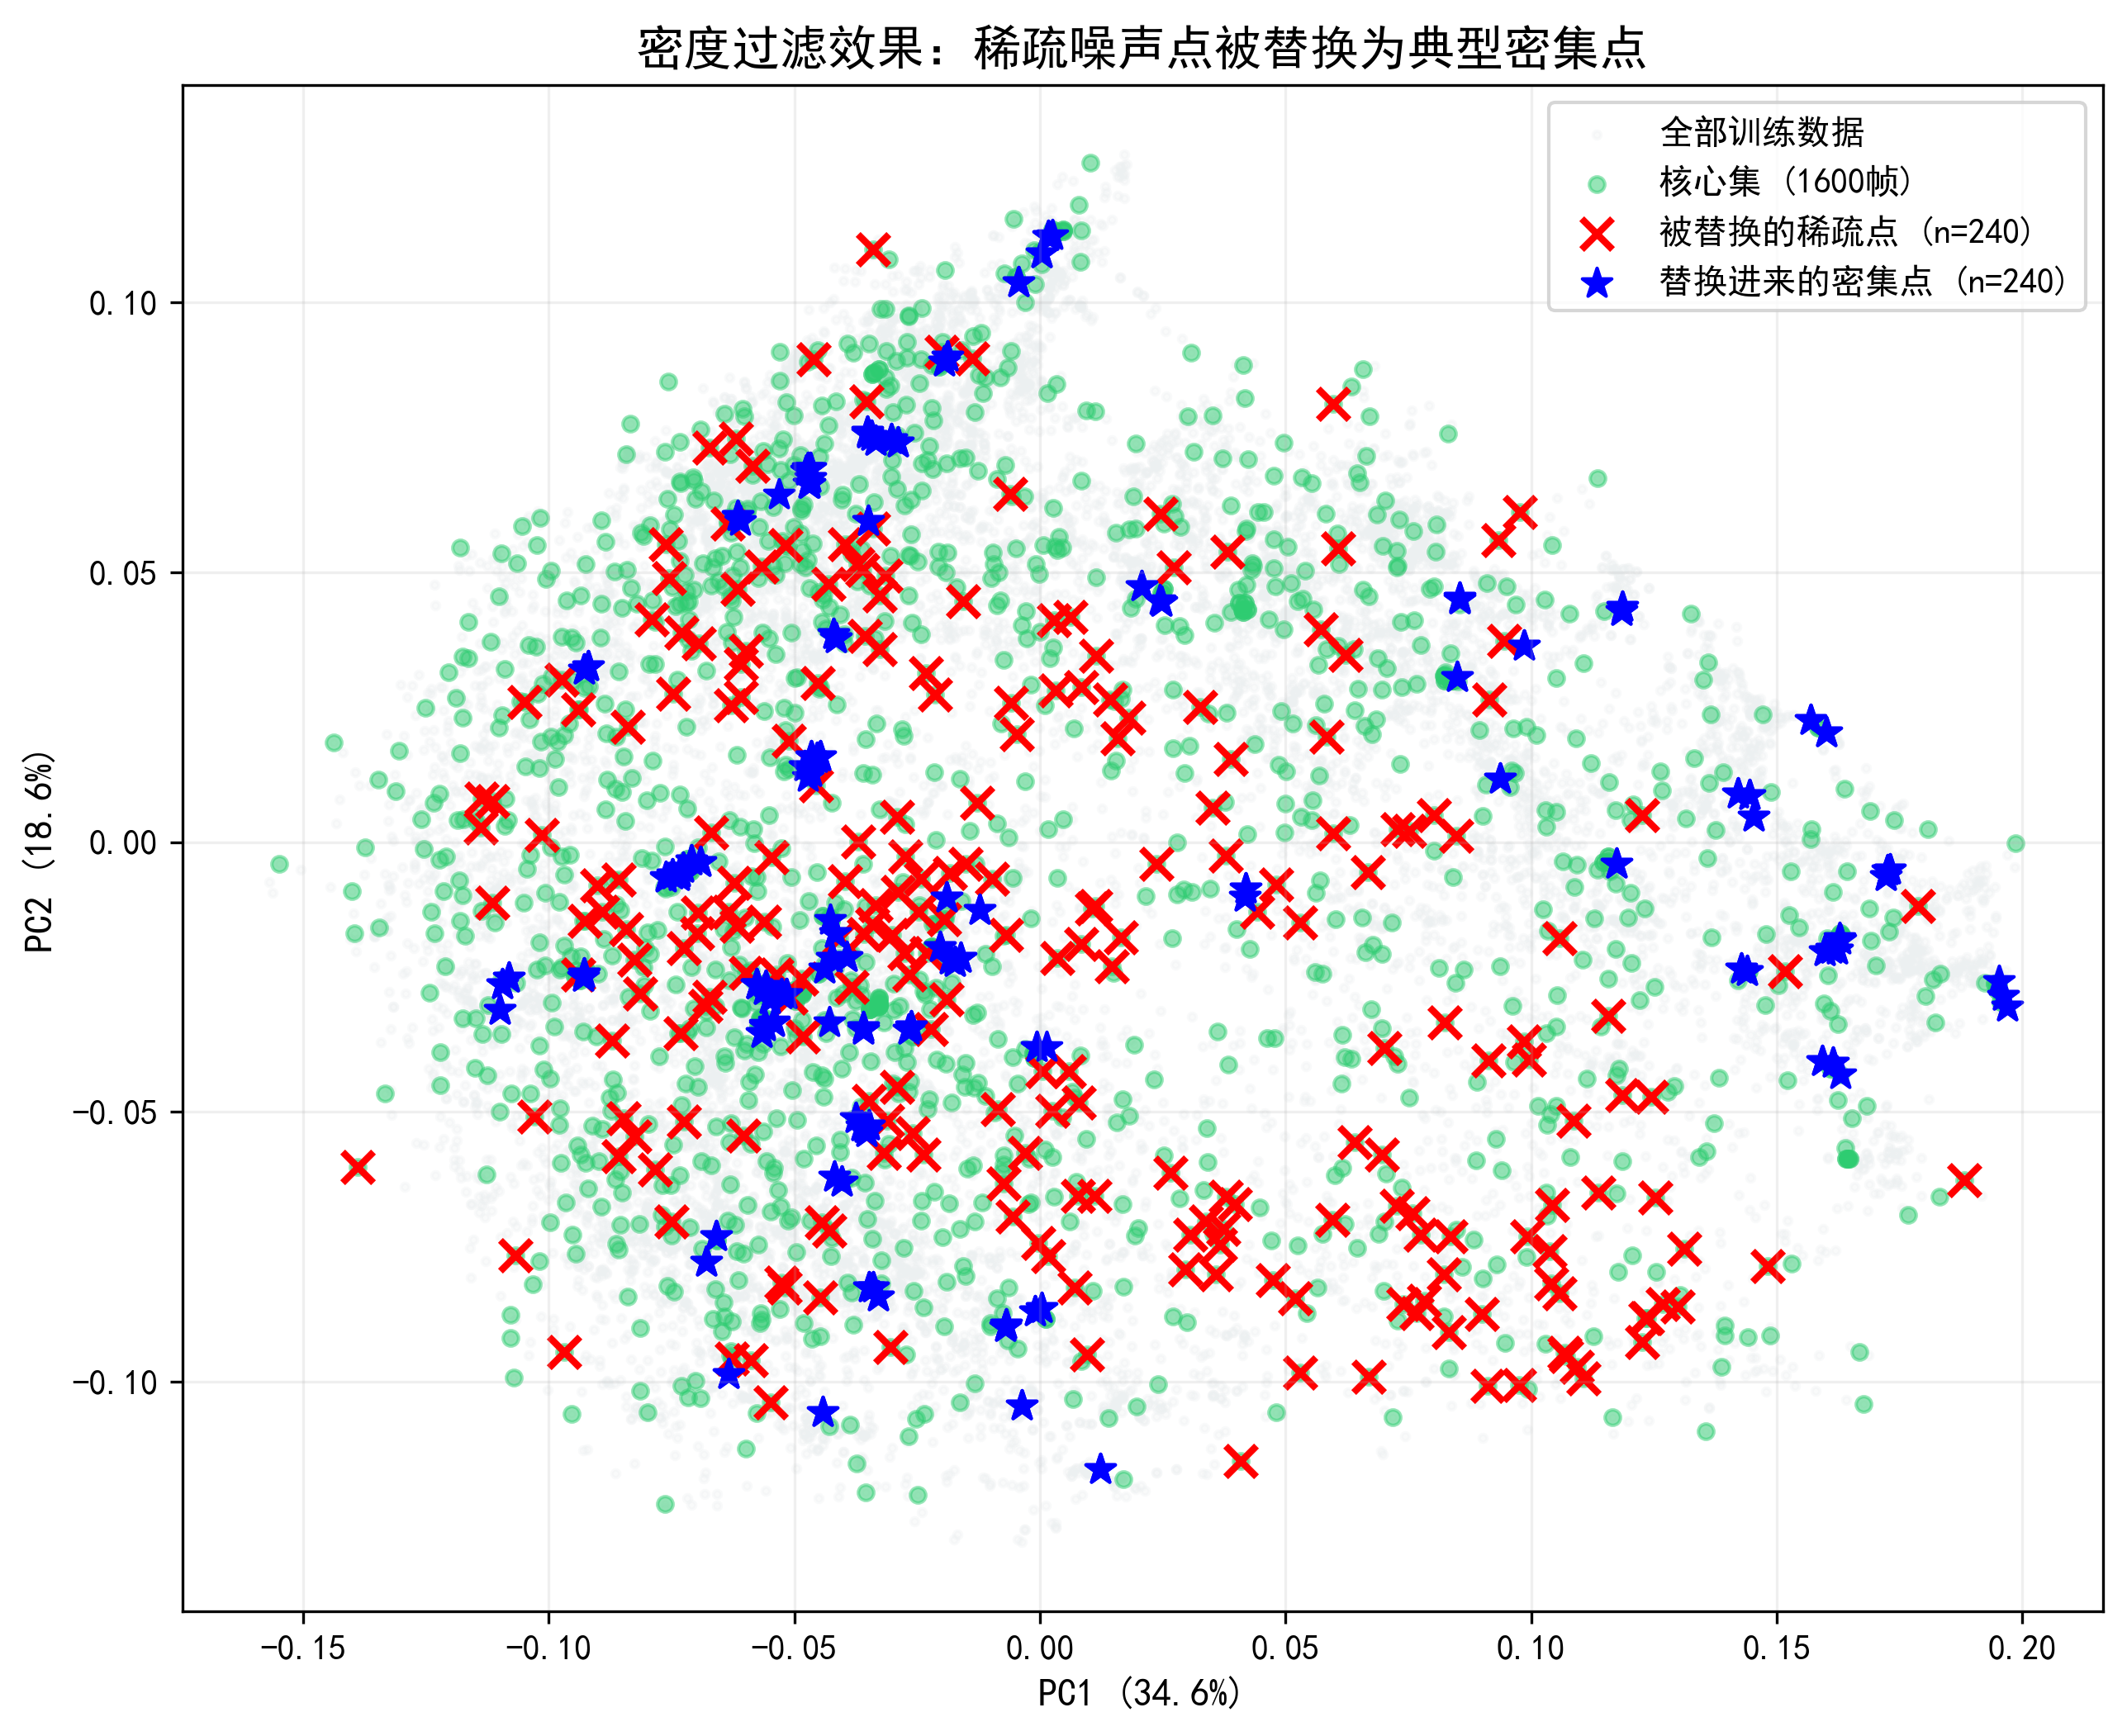
\includegraphics[width=0.75\textwidth]{fig7_density_replacement}
    \caption{密度替换效果散点图}
    \label{fig:density_replacement}
\end{figure}

\begin{figure}[H]
    \centering
    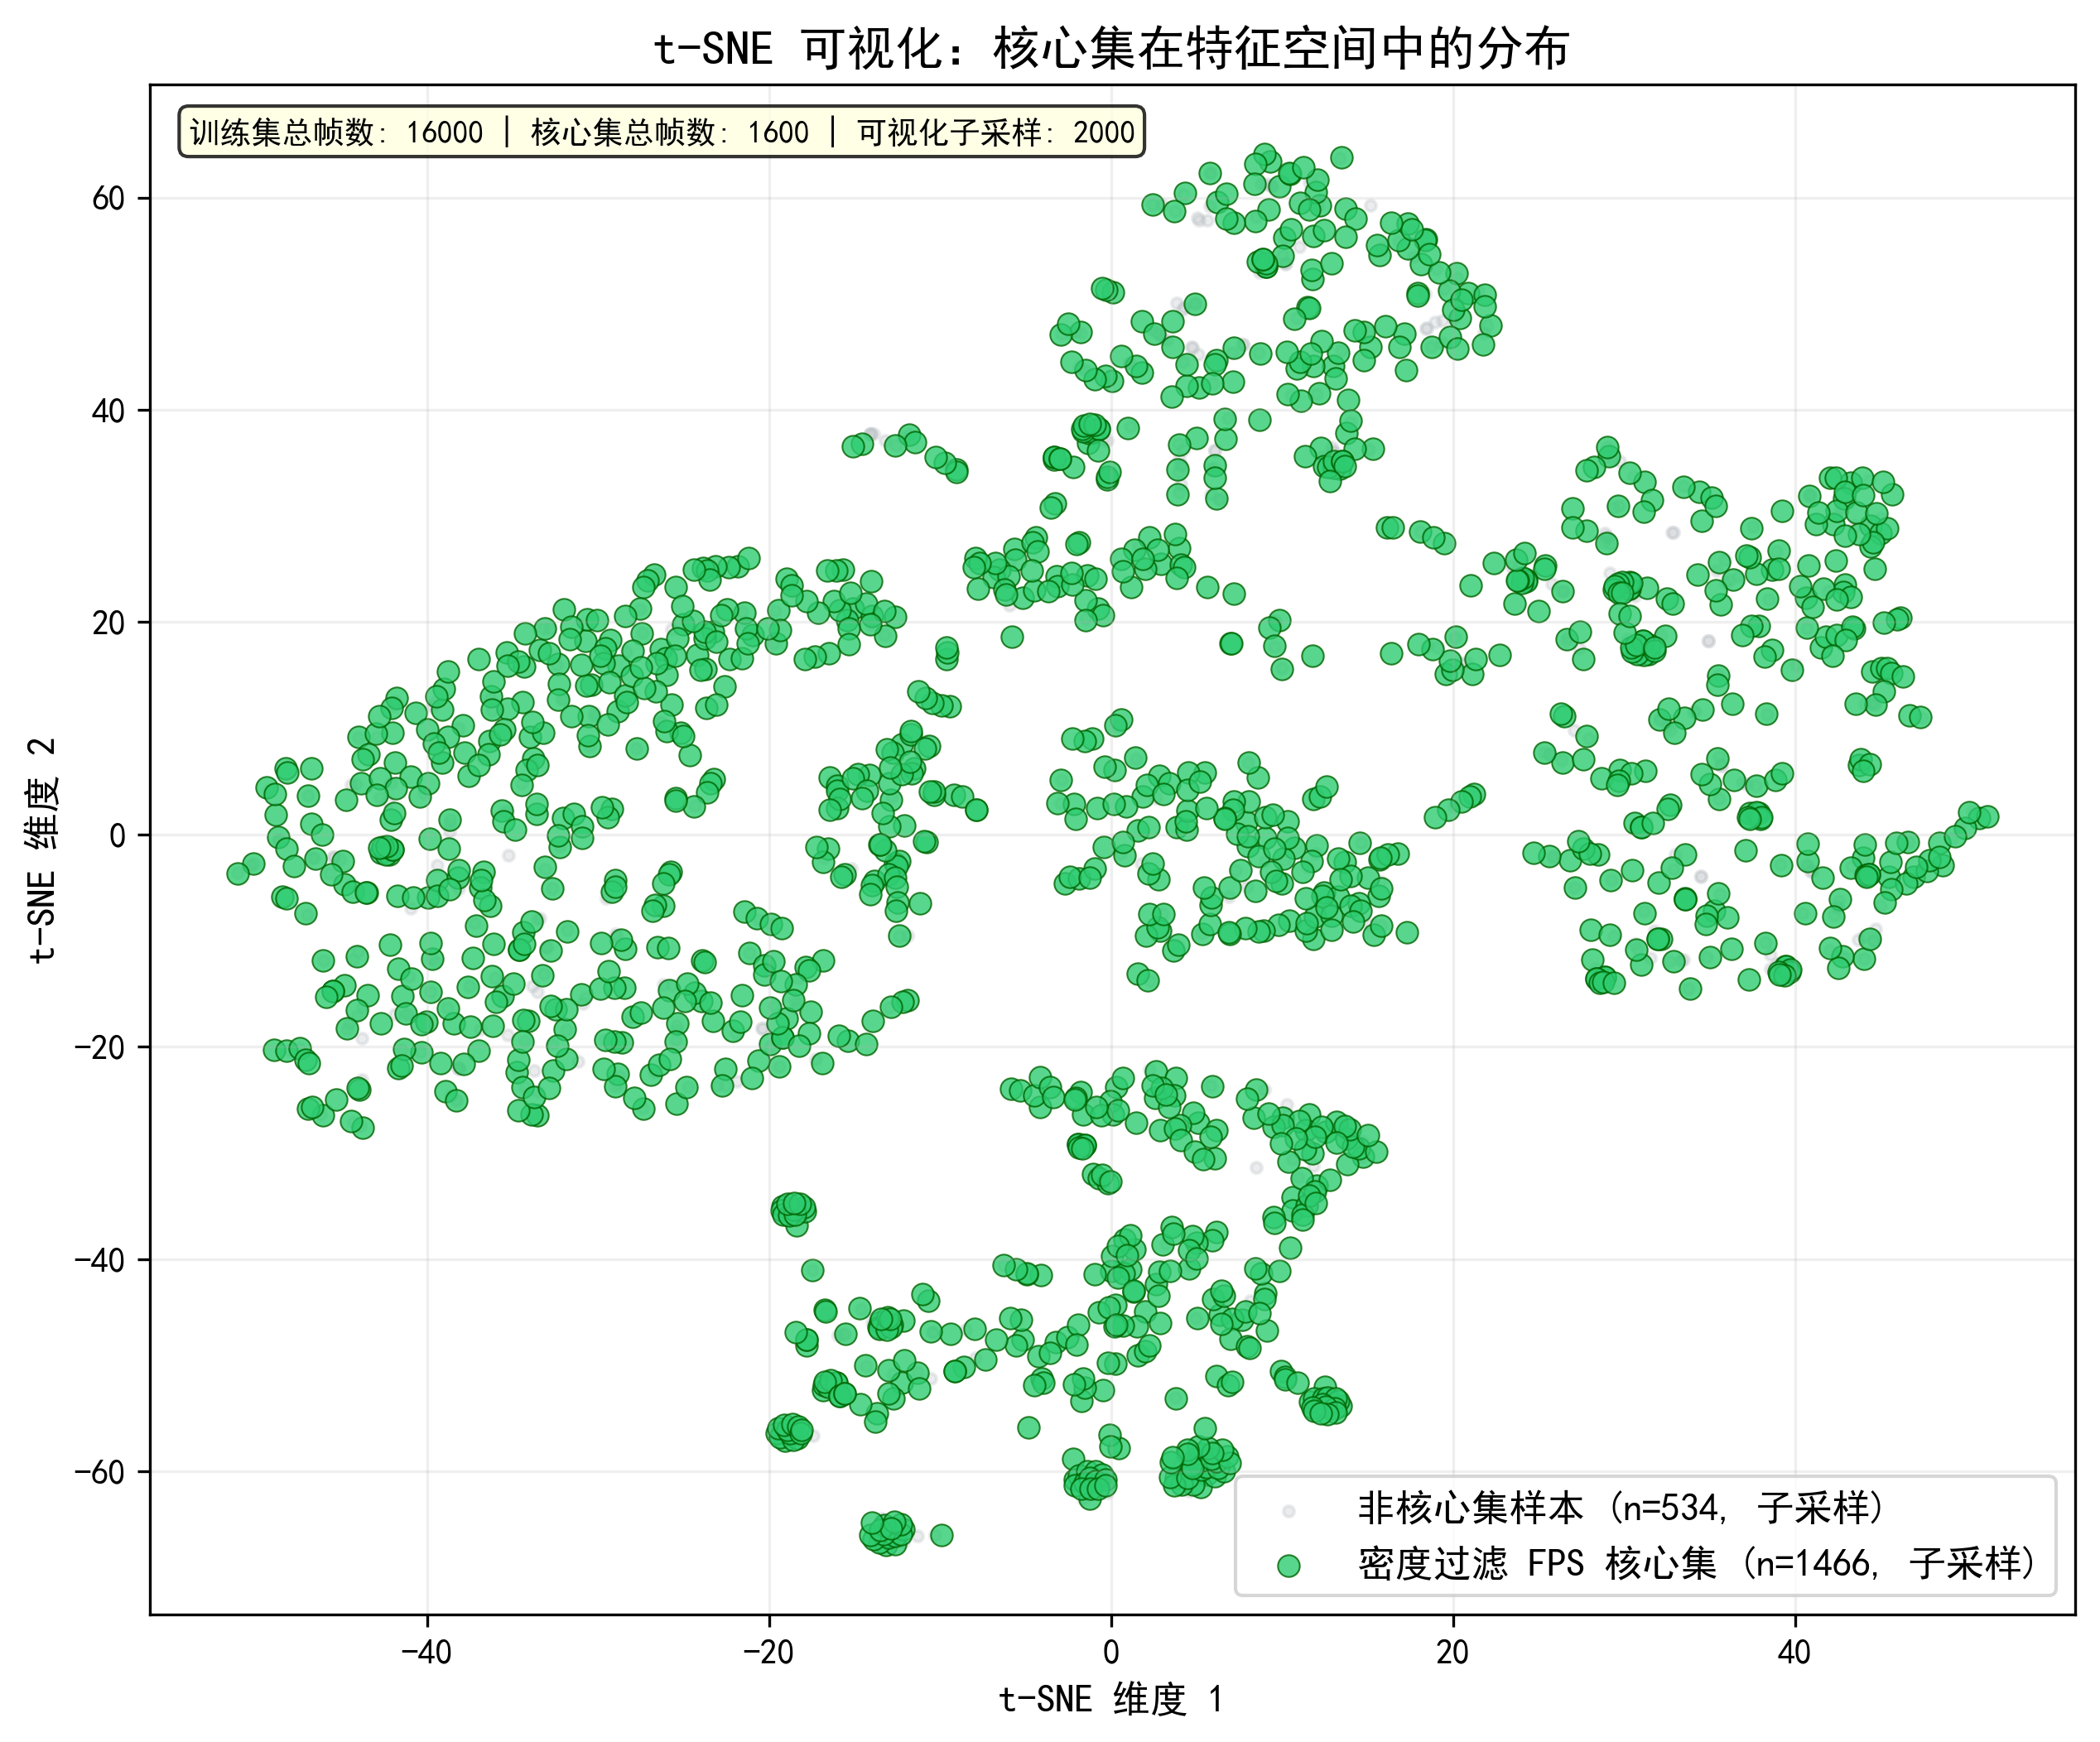
\includegraphics[width=0.75\textwidth]{fig3_tsne_coreset}
    \caption{t-SNE 可视化：密度过滤 FPS（红）均匀覆盖，随机采样（蓝）聚集于高密度区}
    \label{fig:tsne}
\end{figure}

\subsubsection{filter\_ratio 的 U 型曲线}

0.05 修正不足（0.004196），0.15 最优 sweet spot（0.003792），0.25 严重过度（0.004840）。过度替换会削弱 FPS 的空间覆盖优势，把"远但不孤立"的好点也替换掉，退化为随机采样（图~\ref{fig:filter_ratio}）。U 型曲线揭示了一个普遍规律：后处理必须是"微调"而非"重构"。

\begin{figure}[H]
    \centering
    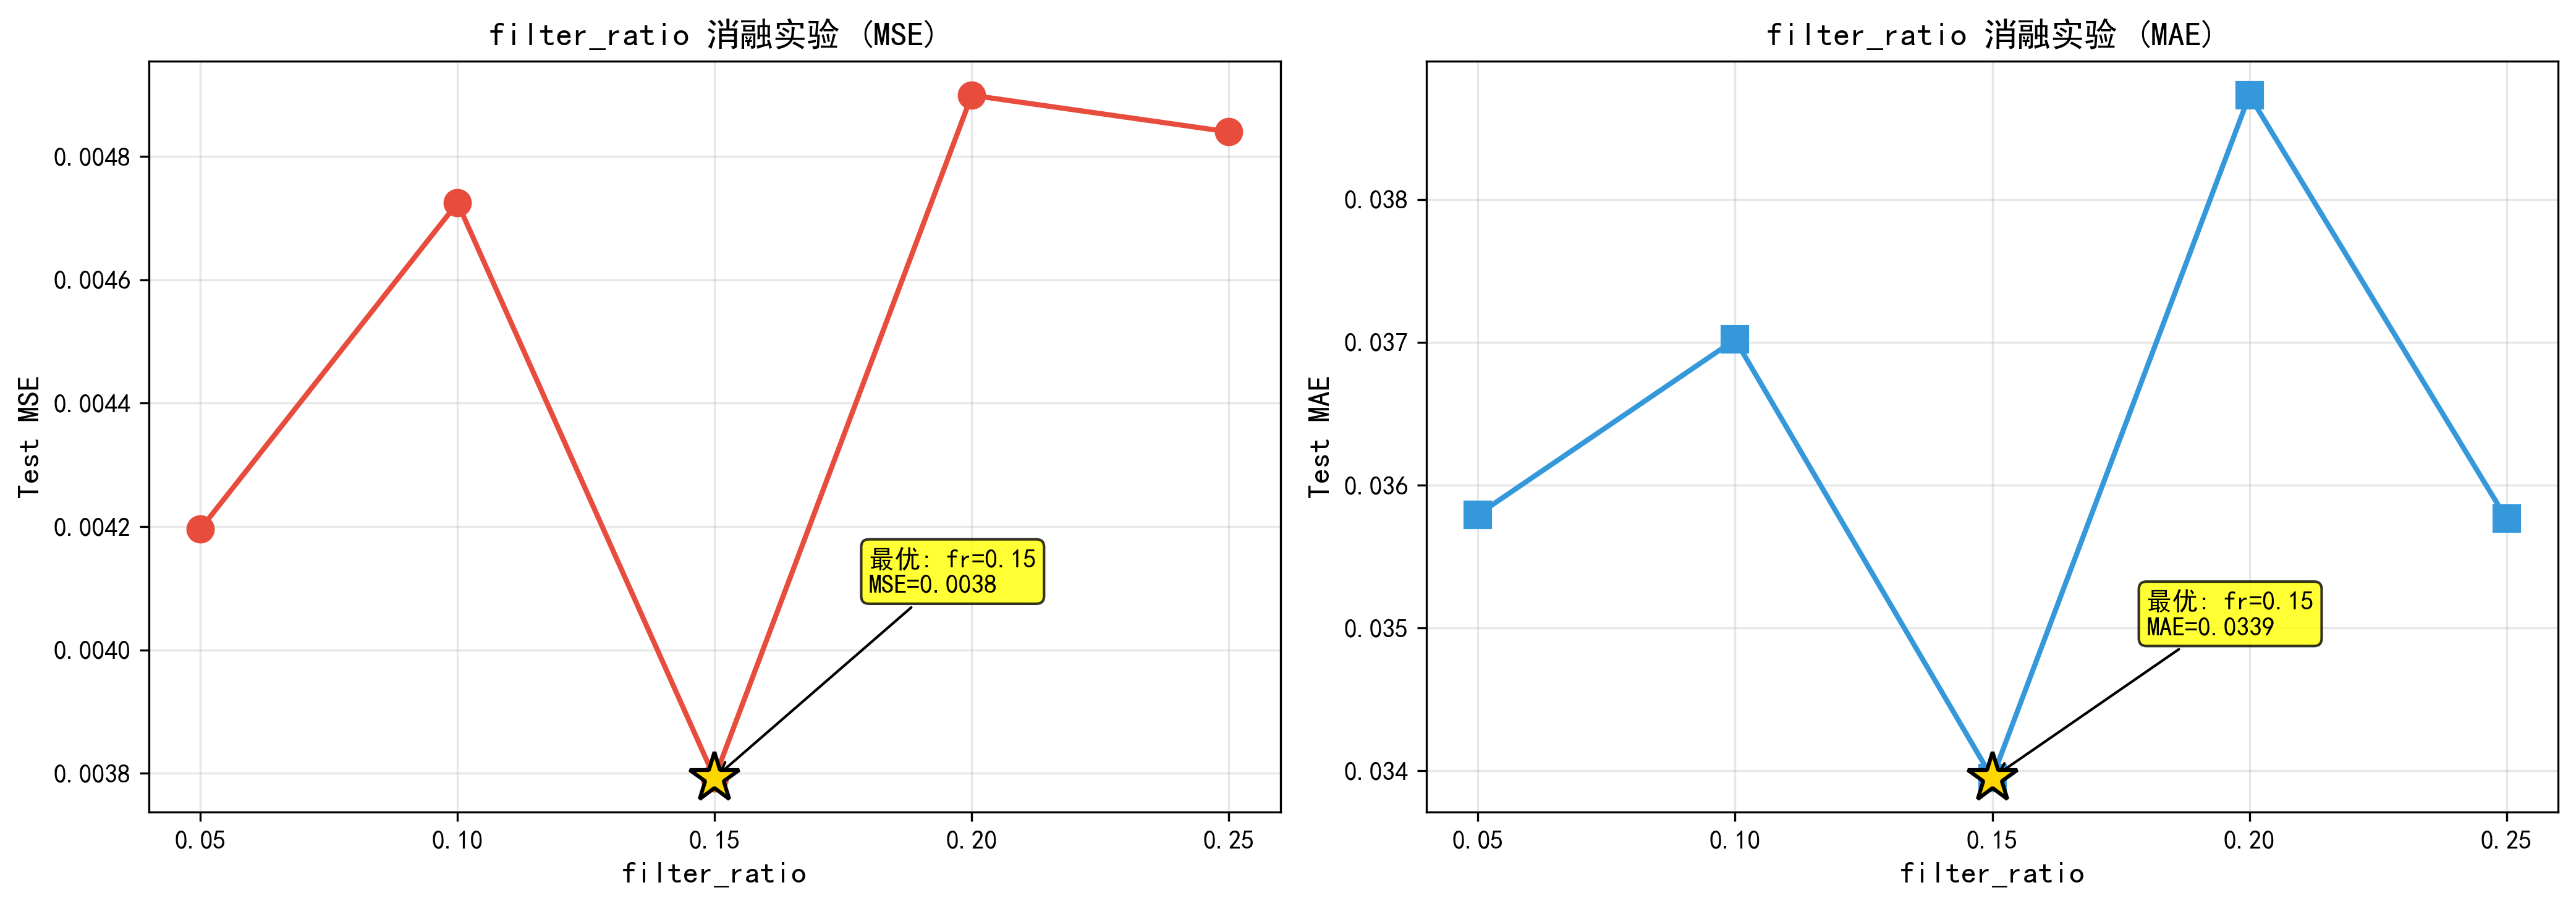
\includegraphics[width=0.95\textwidth]{fig2_filter_ratio_ablation}
    \caption{filter\_ratio 消融曲线。0.15 为最优 sweet spot}
    \label{fig:filter_ratio}
\end{figure}

\subsection{两种成功方法的对比}

表~\ref{tab:method_comparison}从覆盖机制、去噪机制、复杂度、信息损失和最终精度五个维度对比了两种成功方法。

\begin{table}[htbp]
\centering
\caption{自适应聚类筛选与密度过滤 FPS 的对比}
\label{tab:method_comparison}
\begin{tabular}{@{}lcc@{}}
\toprule
\textbf{维度} & \textbf{自适应聚类 + PCA} & \textbf{密度过滤 FPS} \\
\midrule
覆盖机制 & K-Means 间接覆盖 & FPS 直接距离覆盖 \\
去噪机制 & PCA 线性投影 & k-NN 局部密度过滤 \\
复杂度 & 高（3 层） & 中（2 层） \\
信息损失 & PCA 可能损失判别信息 & 无投影，原始特征直接计算 \\
Test MSE & 0.003835 & \textbf{0.003792} \\
\bottomrule
\end{tabular}
\end{table}

\textbf{覆盖机制}是两者最根本的差异。自适应聚类通过 K-Means 先将特征空间划分为 533 个簇，再在簇内按"远且小"的原则选择代表帧。这种"簇 $
ightarrow$ 代表"的间接近似依赖一个关键假设：簇边界与任务语义边界对齐。然而在本任务中，CLIP 视觉特征空间的簇结构由预训练模型决定，与机器人动作预测的目标并不完全一致。密度过滤 FPS 则放弃了"簇"这一中间抽象，直接在原始特征空间优化最大最小距离覆盖，目标函数与最终任务更直接对齐。

\textbf{去噪机制}的差异进一步放大了这一优势。PCA 400d 虽然有效去除了干扰 K-Means 的噪声方向，但线性投影本质上是"有损压缩"——在丢弃噪声的同时也压缩了判别信息。而密度过滤的 k-NN 局部密度估计直接在原始 768d 特征空间操作，不经过任何投影，只对边缘孤立点做温和替换，信息损失更小。

\textbf{复杂度}上，自适应聚类需要三层pipeline（PCA 降维、K-Means 聚类、动态保底+全局补齐），每层都有超参数；密度过滤 FPS 只有两层（FPS 选点、k-NN 密度替换），结构更简洁。

\textbf{结论}：两种方法都验证了"覆盖稀疏区"这一核心直觉，但密度过滤 FPS 以更直接、更简洁的方式实现了它。这揭示了一个普遍规律：在核心集选择中，目标函数与最终任务的对齐度比算法复杂度更重要。精准的直接操作优于多层间接近似。


% ==================== 5. 融合实验 ====================
\section{融合实验：为什么单一全局最优 $>$ 任何融合}
\label{sec:fusion}

\subsection{实验动机}

直觉告诉我们：两种互补方法融合可以取长补短。密度过滤 FPS 保证几何覆盖，自适应聚类筛选捕捉语义稀疏性，两者结合似乎应该更好。然而，18 个融合实验（5 种架构 $\times$ 多种参数配置 + 预测编码的 4 种改进尝试）无一超越单一最优。

\subsection{五种融合思路及失败原因}

\begin{figure}[htbp]
    \centering
    \begin{subfigure}[b]{0.32\textwidth}
        \centering
        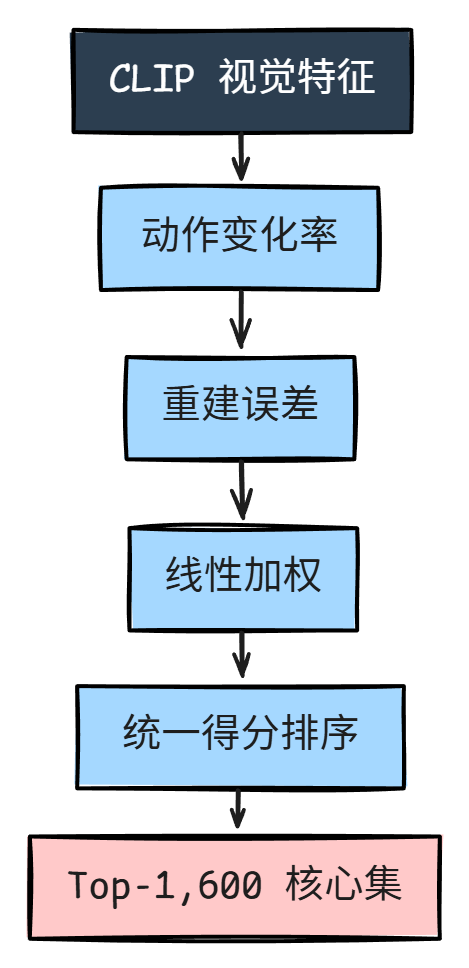
\includegraphics[width=\textwidth]{figE_fusion_score.png}
        \caption{得分融合}
        \label{fig:fusion_score}
    \end{subfigure}
    \hfill
    \begin{subfigure}[b]{0.32\textwidth}
        \centering
        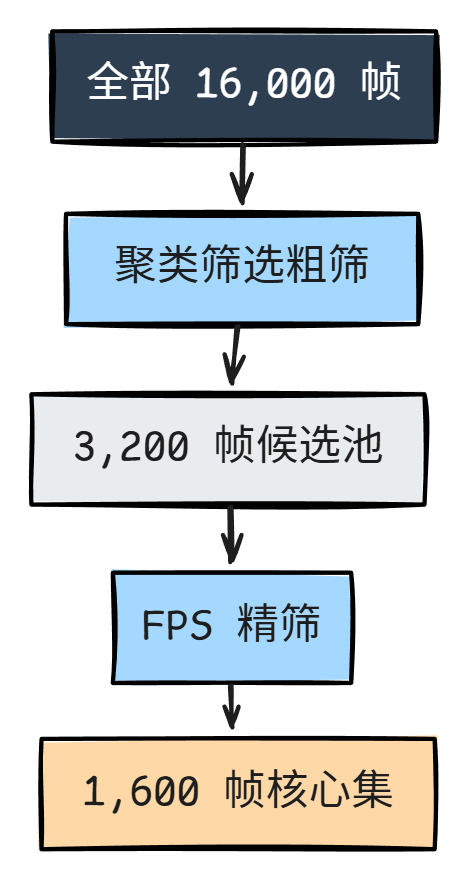
\includegraphics[width=\textwidth]{figE_fusion_hierarchical.png}
        \caption{分层融合}
        \label{fig:fusion_hierarchical}
    \end{subfigure}
    \hfill
    \begin{subfigure}[b]{0.32\textwidth}
        \centering
        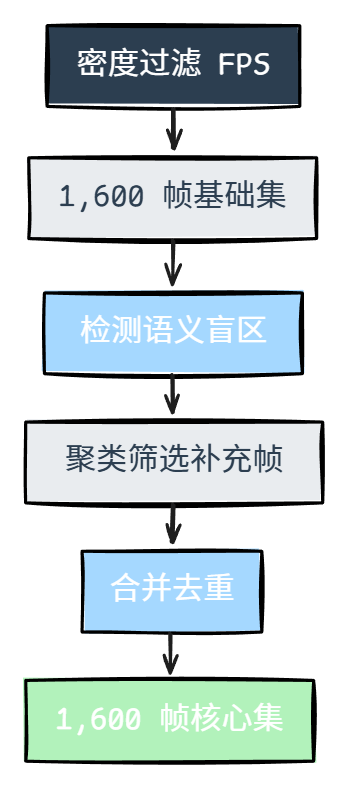
\includegraphics[width=\textwidth]{figE_fusion_complementary.png}
        \caption{互补融合}
        \label{fig:fusion_complementary}
    \end{subfigure}
    
    \vspace{0.5em}
    
    \hspace*{0.16\textwidth}
    \begin{subfigure}[b]{0.32\textwidth}
        \centering
        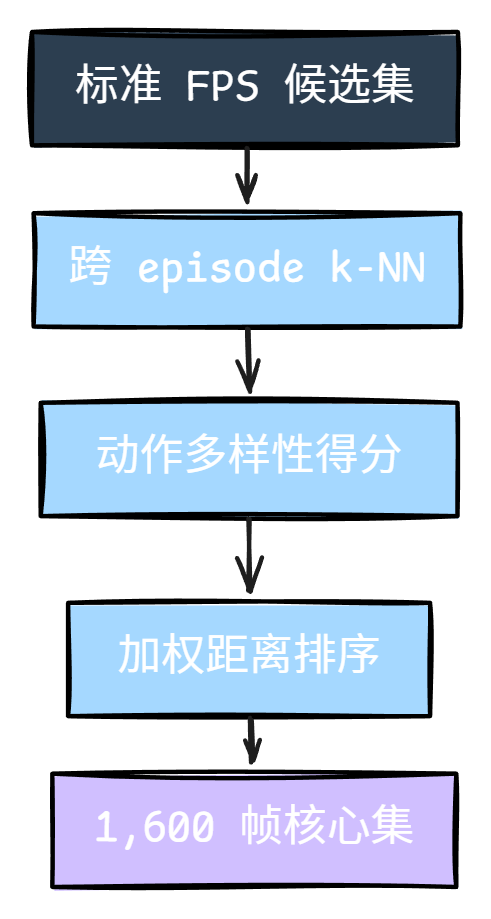
\includegraphics[width=\textwidth]{figE_fusion_action_aware.png}
        \caption{Action-aware FPS}
        \label{fig:fusion_action_aware}
    \end{subfigure}
    \hfill
    \begin{subfigure}[b]{0.32\textwidth}
        \centering
        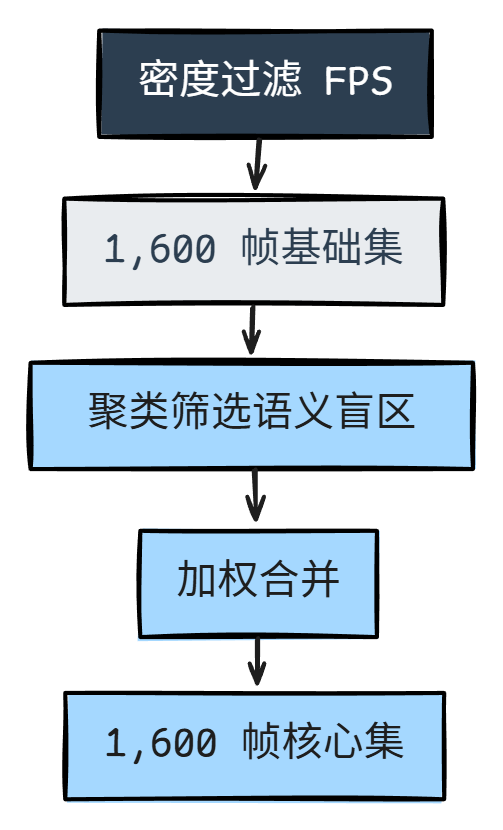
\includegraphics[width=\textwidth]{figE_fusion_semantic_density.png}
        \caption{语义-密度联合}
        \label{fig:fusion_semantic_density}
    \end{subfigure}
    \hspace*{0.16\textwidth}
    
    \caption{五种融合思路架构图}
    \label{fig:fusion_architectures}
\end{figure}

\textbf{思路一：得分融合}（图~\ref{fig:fusion_score}）：动机很直观——既然 CLIP 特征捕捉语义、动作变化率捕捉时序、重建误差捕捉压缩难度，三者线性加权应该能综合多种冗余信号。具体实现：对每帧分别计算 FPS 几何得分、动作变化率得分、AE 重建误差得分，归一化后按 $s = \alpha s_{\text{fps}} + \beta s_{\text{motion}} + \gamma s_{\text{recon}}$ 加权求和，取 Top-1,600。


\textbf{失败}：三种信号并非独立维度。CLIP 语义离群帧和 FPS 几何离群帧在特征空间中往往指向同一批边缘点，而 AE 重建误差在这类边缘点上也偏高。线性加权没有实现"取长补短"，反而对这些边缘点进行了双重甚至三重强调，把噪声放大为"高价值样本"。最优 MSE = 0.005434。

\textbf{思路二：分层融合}（图~\ref{fig:fusion_hierarchical}）：动机是用聚类筛选做"粗筛"保留语义多样性，再用 FPS 做"精筛"保证几何覆盖。具体实现：先用自适应聚类从 16,000 帧选出 3,200 帧候选池（候选比例 cr=2.0），再在该候选池内运行密度过滤 FPS 精选 1,600 帧。


\textbf{失败}：\textbf{信息漏斗效应}——聚类筛选粗筛过滤掉的有用帧，FPS 精筛无法恢复。粗筛决策是硬性的：每一帧要么进入候选池，要么被永久丢弃。一旦密度过滤 FPS 所需的最优帧在粗筛阶段被过滤掉，后续精筛无论多优秀都无法挽回。最优 MSE = 0.004004。

\textbf{思路三：互补融合}（图~\ref{fig:fusion_complementary}）：动机是 FPS 保证几何覆盖，但可能遗漏语义稀疏区；用聚类筛选补充这些"语义盲区"应该能提升覆盖完整性。具体实现：以密度过滤 FPS 选出的 1,600 帧为基础集，再从聚类筛选中选取 400 帧语义稀疏点，合并后去重得到最终 1,600 帧。


\textbf{失败}：单一最优（FPS）的信息完整性已经足够覆盖动作预测所需的关键状态。补充进来的语义稀疏帧虽然分布独特，但对动作预测任务的贡献接近于零，反而稀释了核心集的质量。最优 MSE = 0.004429。

\textbf{思路四：Action-aware FPS}（图~\ref{fig:fusion_action_aware}）：动机是在 FPS 的几何覆盖基础上，加入动作多样性约束，避免选到动作相似的帧。具体实现：标准 FPS 选出候选集后，对每个候选点计算跨 Episode 的 k-NN 动作多样性得分，用该得分加权 FPS 距离，重新排序取 Top-1,600。


\textbf{失败}：跨 Episode 的 k-NN 动作多样性度量失真。不同 Episode 的起始姿态、速度、光照存在系统性差异，导致"动作相似"的判断标准不一致；同时动作信号与视觉特征信号不正交，加权过程相互干扰。最优 MSE = 0.004040。

\textbf{思路五：语义-密度联合}（图~\ref{fig:fusion_semantic_density}）：动机是将聚类筛选的"稀疏簇偏好"与 FPS 的"几何覆盖"联合成一个统一得分。具体实现：对每帧同时计算 FPS 几何得分和聚类语义稀缺得分（基于簇大小的倒数），加权合并后排序。


\textbf{失败}：语义稀有 $\neq$ 动作预测价值。聚类筛选眼中的"语义盲区"往往是对动作预测无贡献的噪声区域——它们在 CLIP 特征空间中独特，但在动作空间中没有对应的变化。把这些帧加入核心集引入了方差。最优 MSE = 0.004079。

\subsection{融合失败的三层原因分析}

图~\ref{fig:fusion_failure}直观展示了所有融合方法的失败：没有任何融合能超越单一最优（0.003792），最佳融合（分层融合 0.004004）仍有 5.6\% 差距。失败可归因于三层机制问题：

\begin{figure}[H]
    \centering
    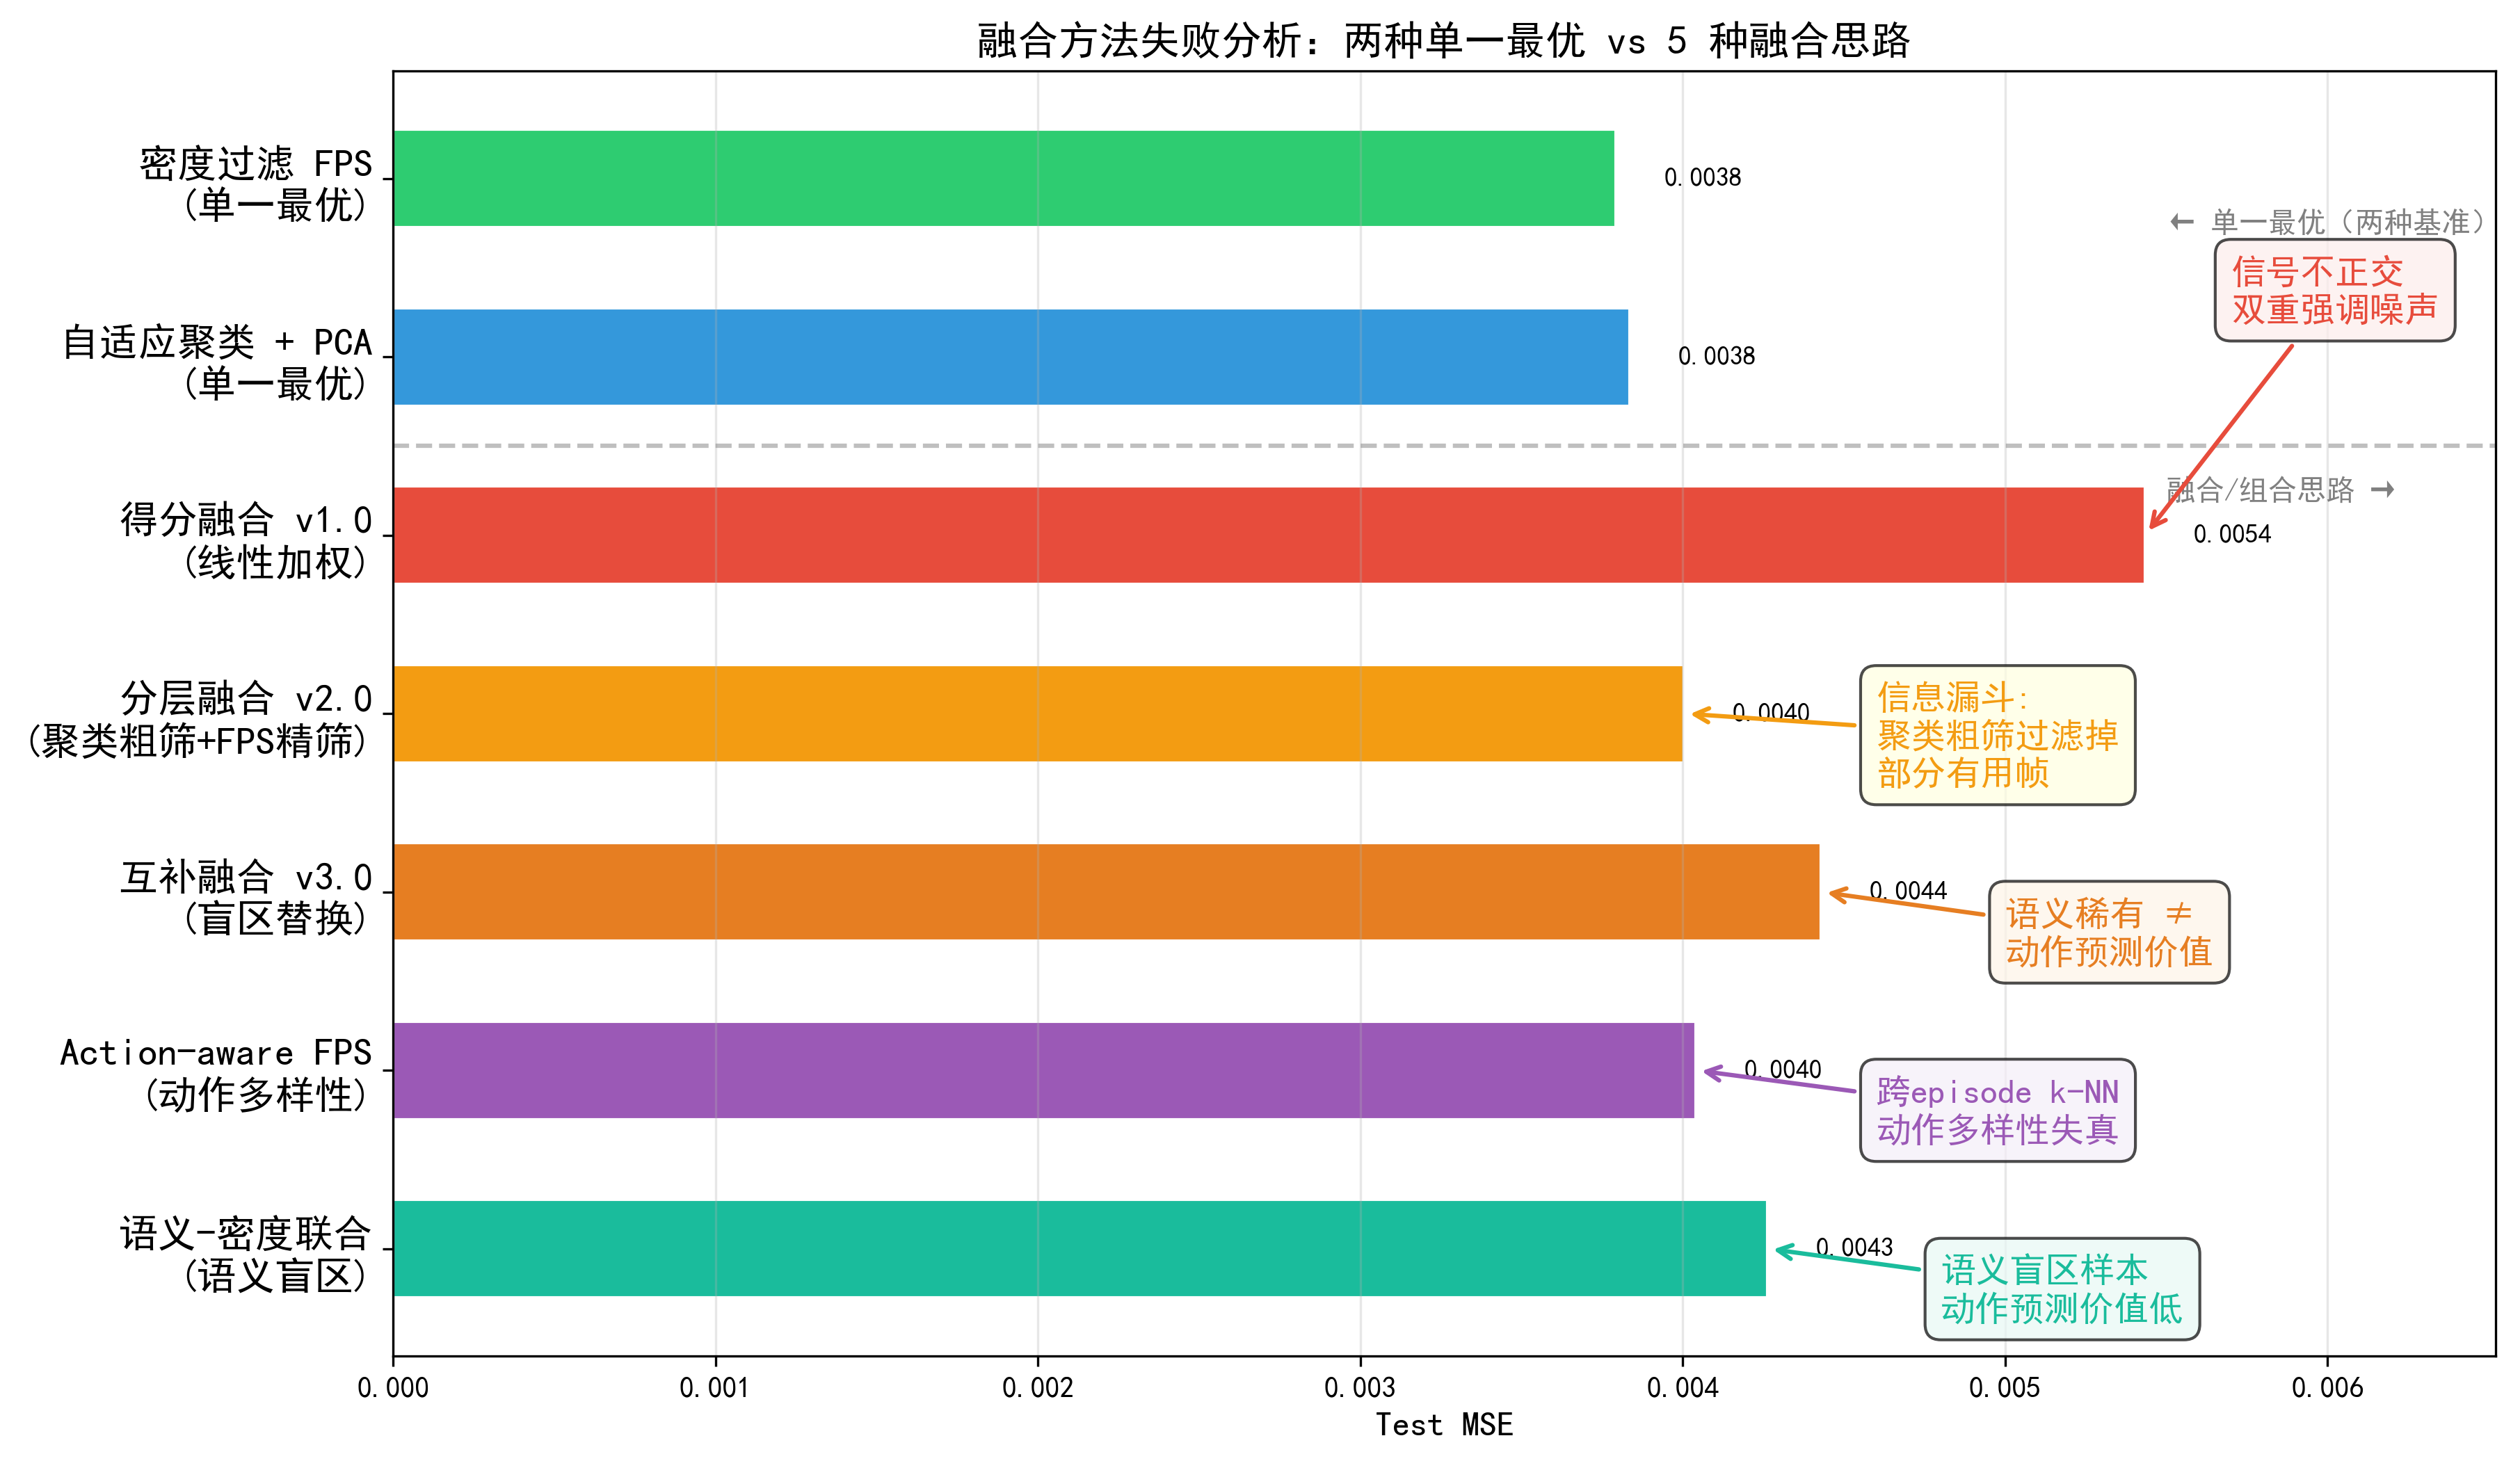
\includegraphics[width=0.95\textwidth]{fig10_fusion_failure}
    \caption{融合方法失败分析柱状图。单一最优（0.003792）显著优于所有融合}
    \label{fig:fusion_failure}
\end{figure}

\textbf{第一层：信号不正交}。得分融合将 CLIP 视觉特征、动作变化率、重建误差三种信号线性加权。问题在于，这三种信号并非独立维度——CLIP 语义离群帧和 FPS 几何离群帧在特征空间中往往指向同一批边缘点。线性加权不仅没有实现"取长补短"，反而对这些边缘点进行了双重甚至三重强调，把噪声放大为"高价值样本"。

\textbf{第二层：信息漏斗效应}。分层融合先用聚类筛选将 16,000 帧压缩到 3,200 帧候选池，再用 FPS 从中精选 1,600 帧。这个结构看似合理，实则存在一个不可修复的信息损失：聚类筛选的决策是硬性的——每一帧要么进入候选池，要么被永久丢弃。一旦密度过滤 FPS 所需的最优帧在粗筛阶段被过滤掉，精筛阶段的 FPS 无论多么优秀都无法恢复它。候选池越小，信息漏斗效应越严重；候选池越大，粗筛本身又失去意义。

\textbf{第三层：信息相关性的上限}。互补融合和语义-密度联合融合试图用聚类筛选补充 FPS 的"语义盲区"。但实验表明，这些所谓盲区往往是对动作预测无贡献的噪声区域。即使能精确识别出语义稀有帧，如果它们与目标动作之间没有统计相关性，补充进去只会引入方差。融合的上限不是算法设计问题，而是信息论问题：两个高度相关的信号源无法通过融合产生超越各自的信息量。

\subsection{核心结论}

融合实验的失败并非源于参数调优不足或架构设计粗糙，而是揭示了核心集选择任务中的一个结构性规律：当单一全局最优方法已经充分利用了与目标任务相关的信息时，任何基于该方法的信息重组或补充都难以产生额外收益。

具体而言，本研究的融合尝试受到三类根本性约束。

\textbf{第一，信息漏斗效应构成多层融合的根本瓶颈。}分层融合通过聚类筛选粗筛构建候选池，再经 FPS 精筛得到最终核心集。然而，粗筛阶段的决策是硬性的——每一帧要么进入候选池，要么被永久丢弃。一旦密度过滤 FPS 所需的最优帧在粗筛阶段被过滤，精筛阶段无论多么优秀都无法恢复。实验中最优分层融合的 MSE 为 0.004004，仍落后于单一最优的 0.003792，差距虽仅 5.6\%，但这 5.6\% 恰恰对应了粗筛阶段丢失的关键信息。

\textbf{第二，信号非正交性限制了加权融合的有效性。}得分融合试图将 CLIP 语义得分、动作变化率得分和重建误差得分线性组合，但这三种信号在特征空间中高度相关：语义离群帧、几何离群帧和重建误差大的帧往往指向同一批边缘点。线性加权不仅未能实现"取长补短"，反而对这些边缘点进行了多重强调，放大了噪声。

\textbf{第三，信息相关性上限决定了互补融合的天花板。}互补融合和语义-密度联合试图补充 FPS 的"语义盲区"，但实验表明，这些盲区中的帧虽然在特征空间分布独特，却与动作预测目标缺乏统计相关性。冗余信号必须满足"与目标正交互补"的条件，否则补充只会引入方差。

综上所述，本研究的 18 个融合实验全部失败，无一超越单一全局最优。这一结果强烈表明：在核心集选择中，与其设计复杂的融合策略，不如精确定义冗余并选择与之匹配的直接优化方法。

% ==================== 6. 实验结果与对比分析 ====================
\section{实验结果与对比分析}
\label{sec:results}

\subsection{全局方法排名}

\begin{table}[htbp]
\centering
\caption{全局方法性能排名（Test MSE，越低越好）}
\label{tab:global_ranking}
\begin{tabular}{@{}clccc@{}}
\toprule
\textbf{排名} & \textbf{方法} & \textbf{冗余定义} & \textbf{Test MSE} & \textbf{vs 随机基线} \\
\midrule
\textbf{1} & \textbf{密度过滤 FPS} & 几何覆盖冗余 & \textbf{0.003792} & \textbf{$\downarrow$47.5\%} \\
\textbf{2} & 自适应聚类 + PCA 去噪 & 分布冗余 & 0.003835 & $\downarrow$47.0\% \\
3 & 分层融合 cr2.0 & 融合 & 0.004004 & $\downarrow$44.6\% \\
4 & 预测编码滑动窗口 & 时序冗余 & 0.005688 & $\downarrow$21.3\% \\
-- & \textbf{随机基线} & -- & \textbf{0.007229} & -- \\
-- & 时序事件边界 & 时序冗余 & 0.008871 & $\uparrow$22.7\% \textcolor{red}{失败} \\
-- & AE 重建误差 & 压缩冗余 & $\sim$0.007 & $\sim$0\% \textcolor{red}{失败} \\
\bottomrule
\end{tabular}
\end{table}

\begin{figure}[htbp]
    \centering
    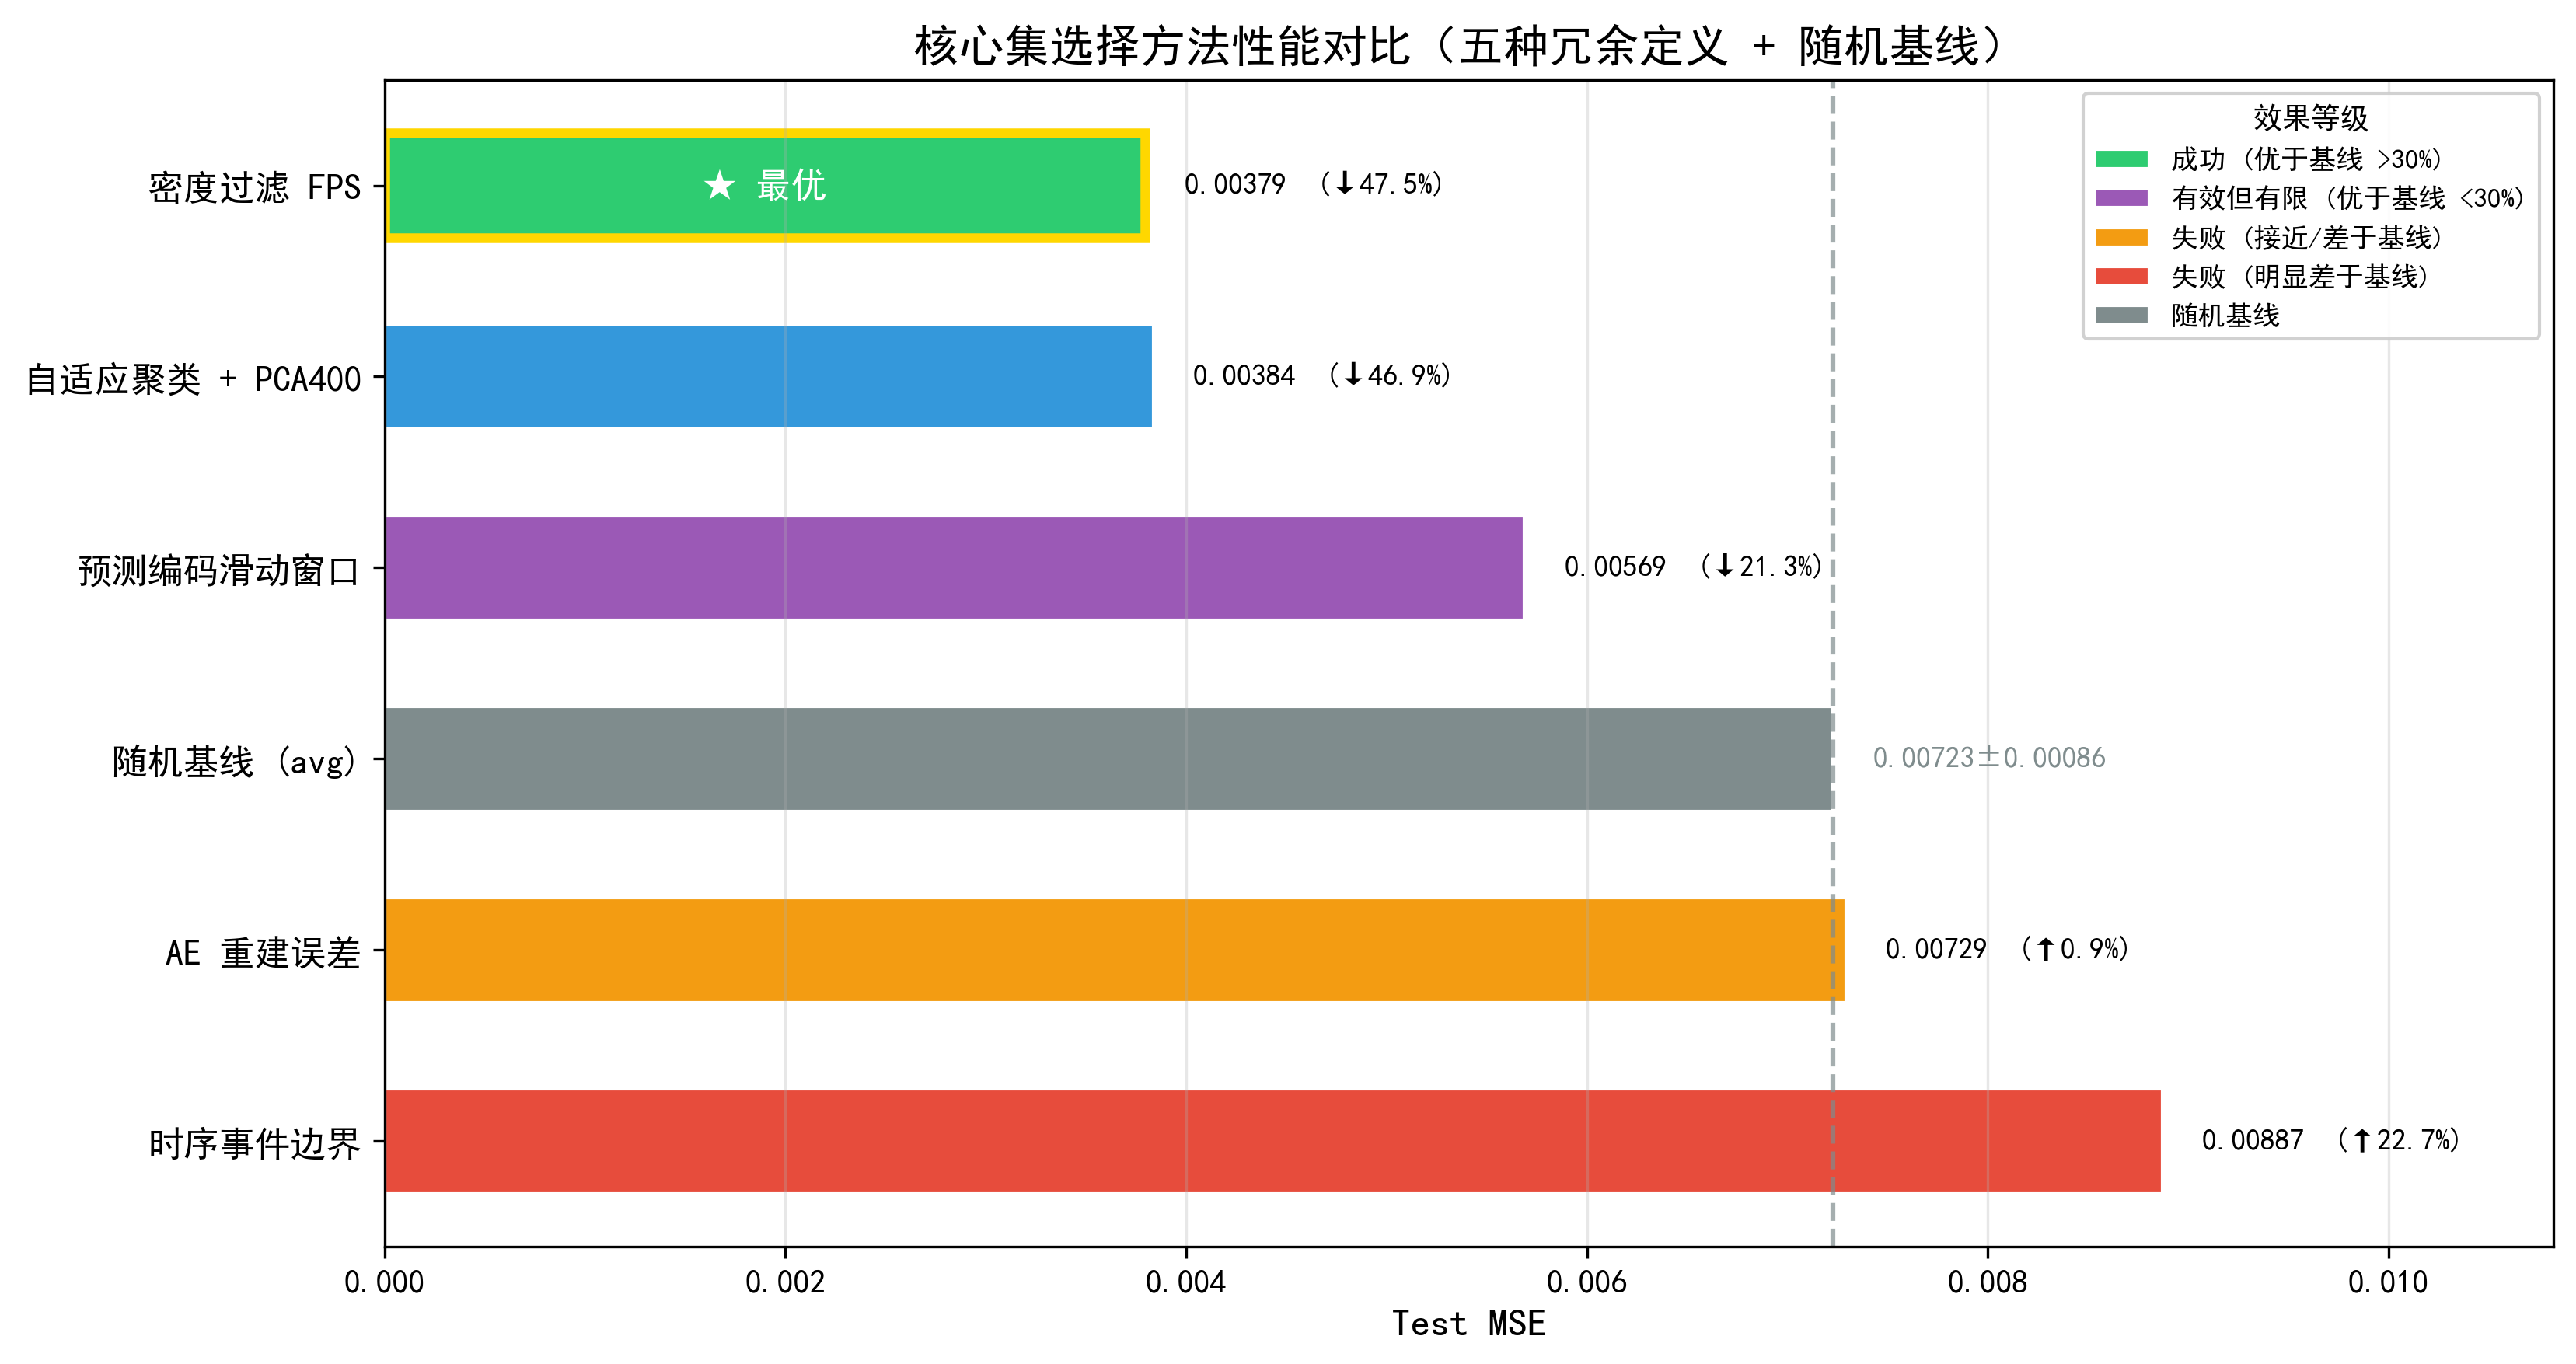
\includegraphics[width=0.85\textwidth]{fig1_method_comparison}
    \caption{全局方法性能对比柱状图。密度过滤 FPS 显著优于所有其他方法}
    \label{fig:method_comparison}
\end{figure}

图~\ref{fig:method_comparison}直观展示了全局方法排名。密度过滤 FPS（0.003792）和自适应聚类筛选 + PCA（0.003835）显著优于随机基线（0.007229），时序方法（0.008871）和 AE 方法（$\sim$0.007）失败。值得强调的是，即使是"失败"的预测编码（0.005688），也较随机基线降低了 21.3\%，说明"可预测 = 冗余"的假设部分成立，只是受限于数据特性未能达到最优。

\subsection{学习曲线对比}

\begin{figure}[htbp]
    \centering
    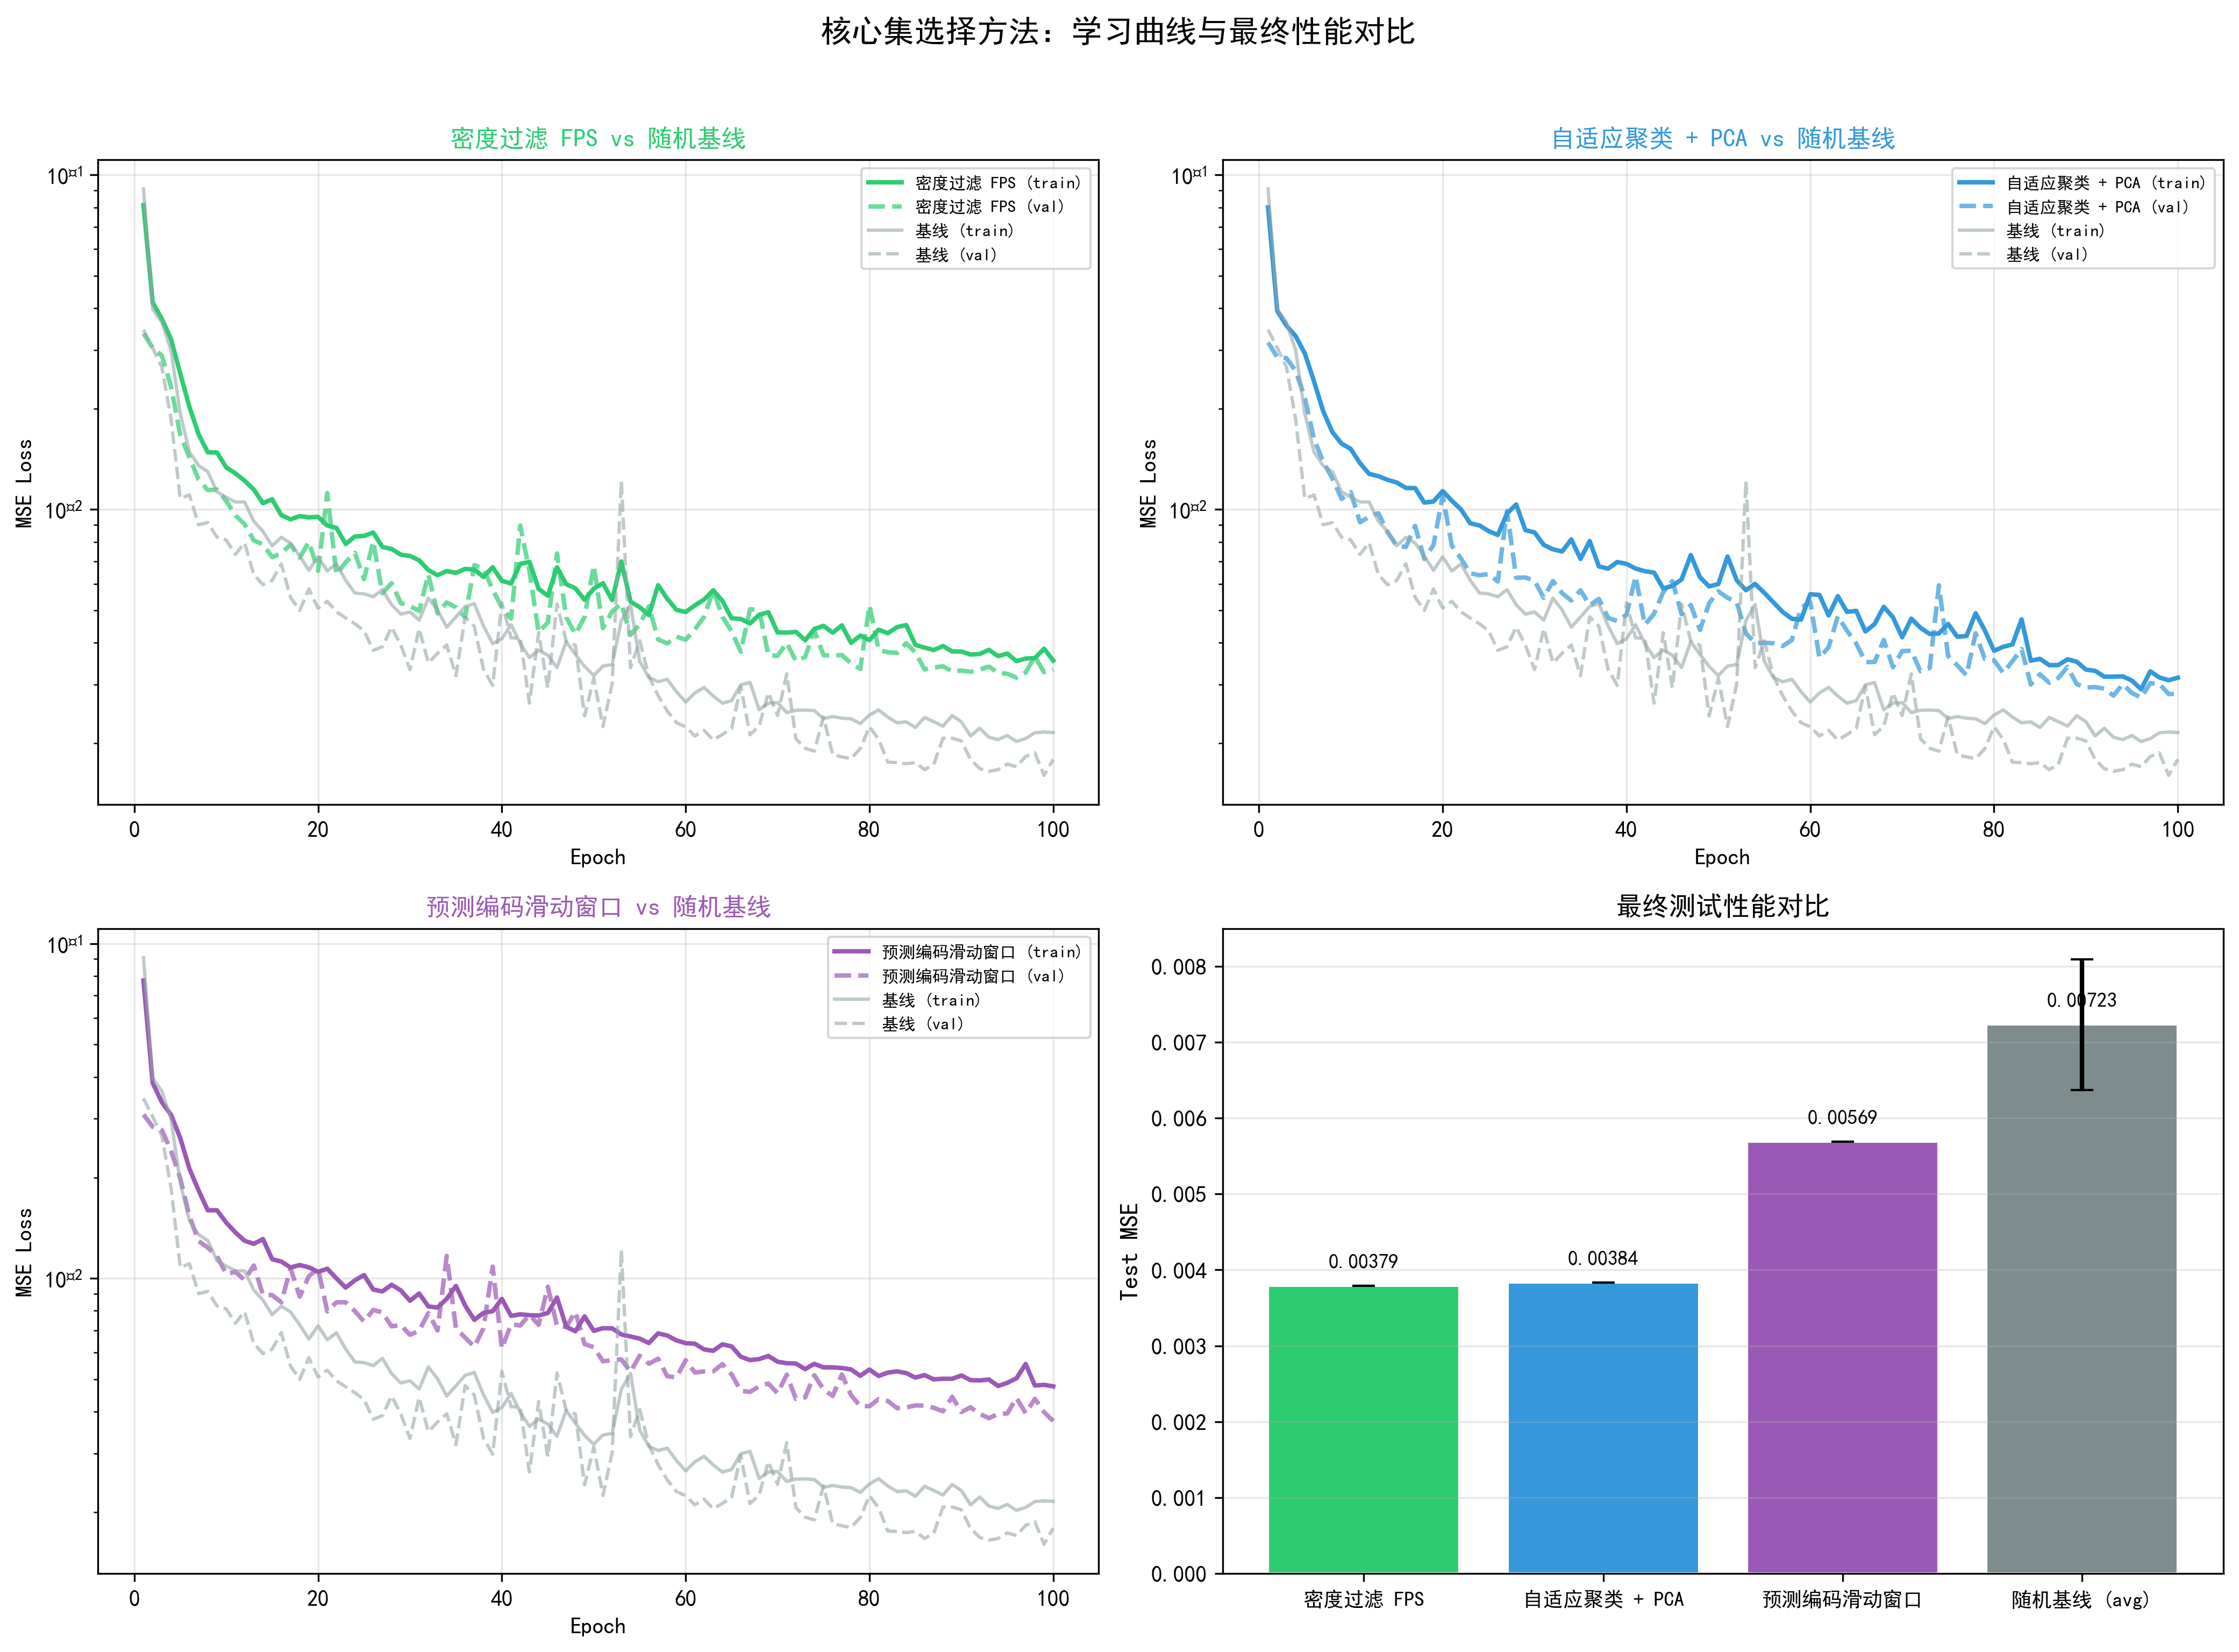
\includegraphics[width=0.95\textwidth]{fig5_learning_curves}
    \caption{学习曲线对比（左上：FPS vs 基线；右上：聚类 vs 基线；左下：预测编码 vs 基线；右下：最终测试性能）}
    \label{fig:learning_curves}
\end{figure}

图~\ref{fig:learning_curves}展示了三种成功方法与随机基线的学习曲线对比。密度过滤 FPS（红色）收敛最快，验证 loss 最低且最稳定；自适应聚类筛选（绿色）次之；预测编码（紫色）收敛速度与基线接近但最终验证 loss 更低；随机基线（蓝色）收敛慢，过拟合风险高。右下角的最终测试性能柱状图再次确认了密度过滤 FPS 的优势。

\subsection{7DoF 每关节误差分析}

\begin{figure}[htbp]
    \centering
    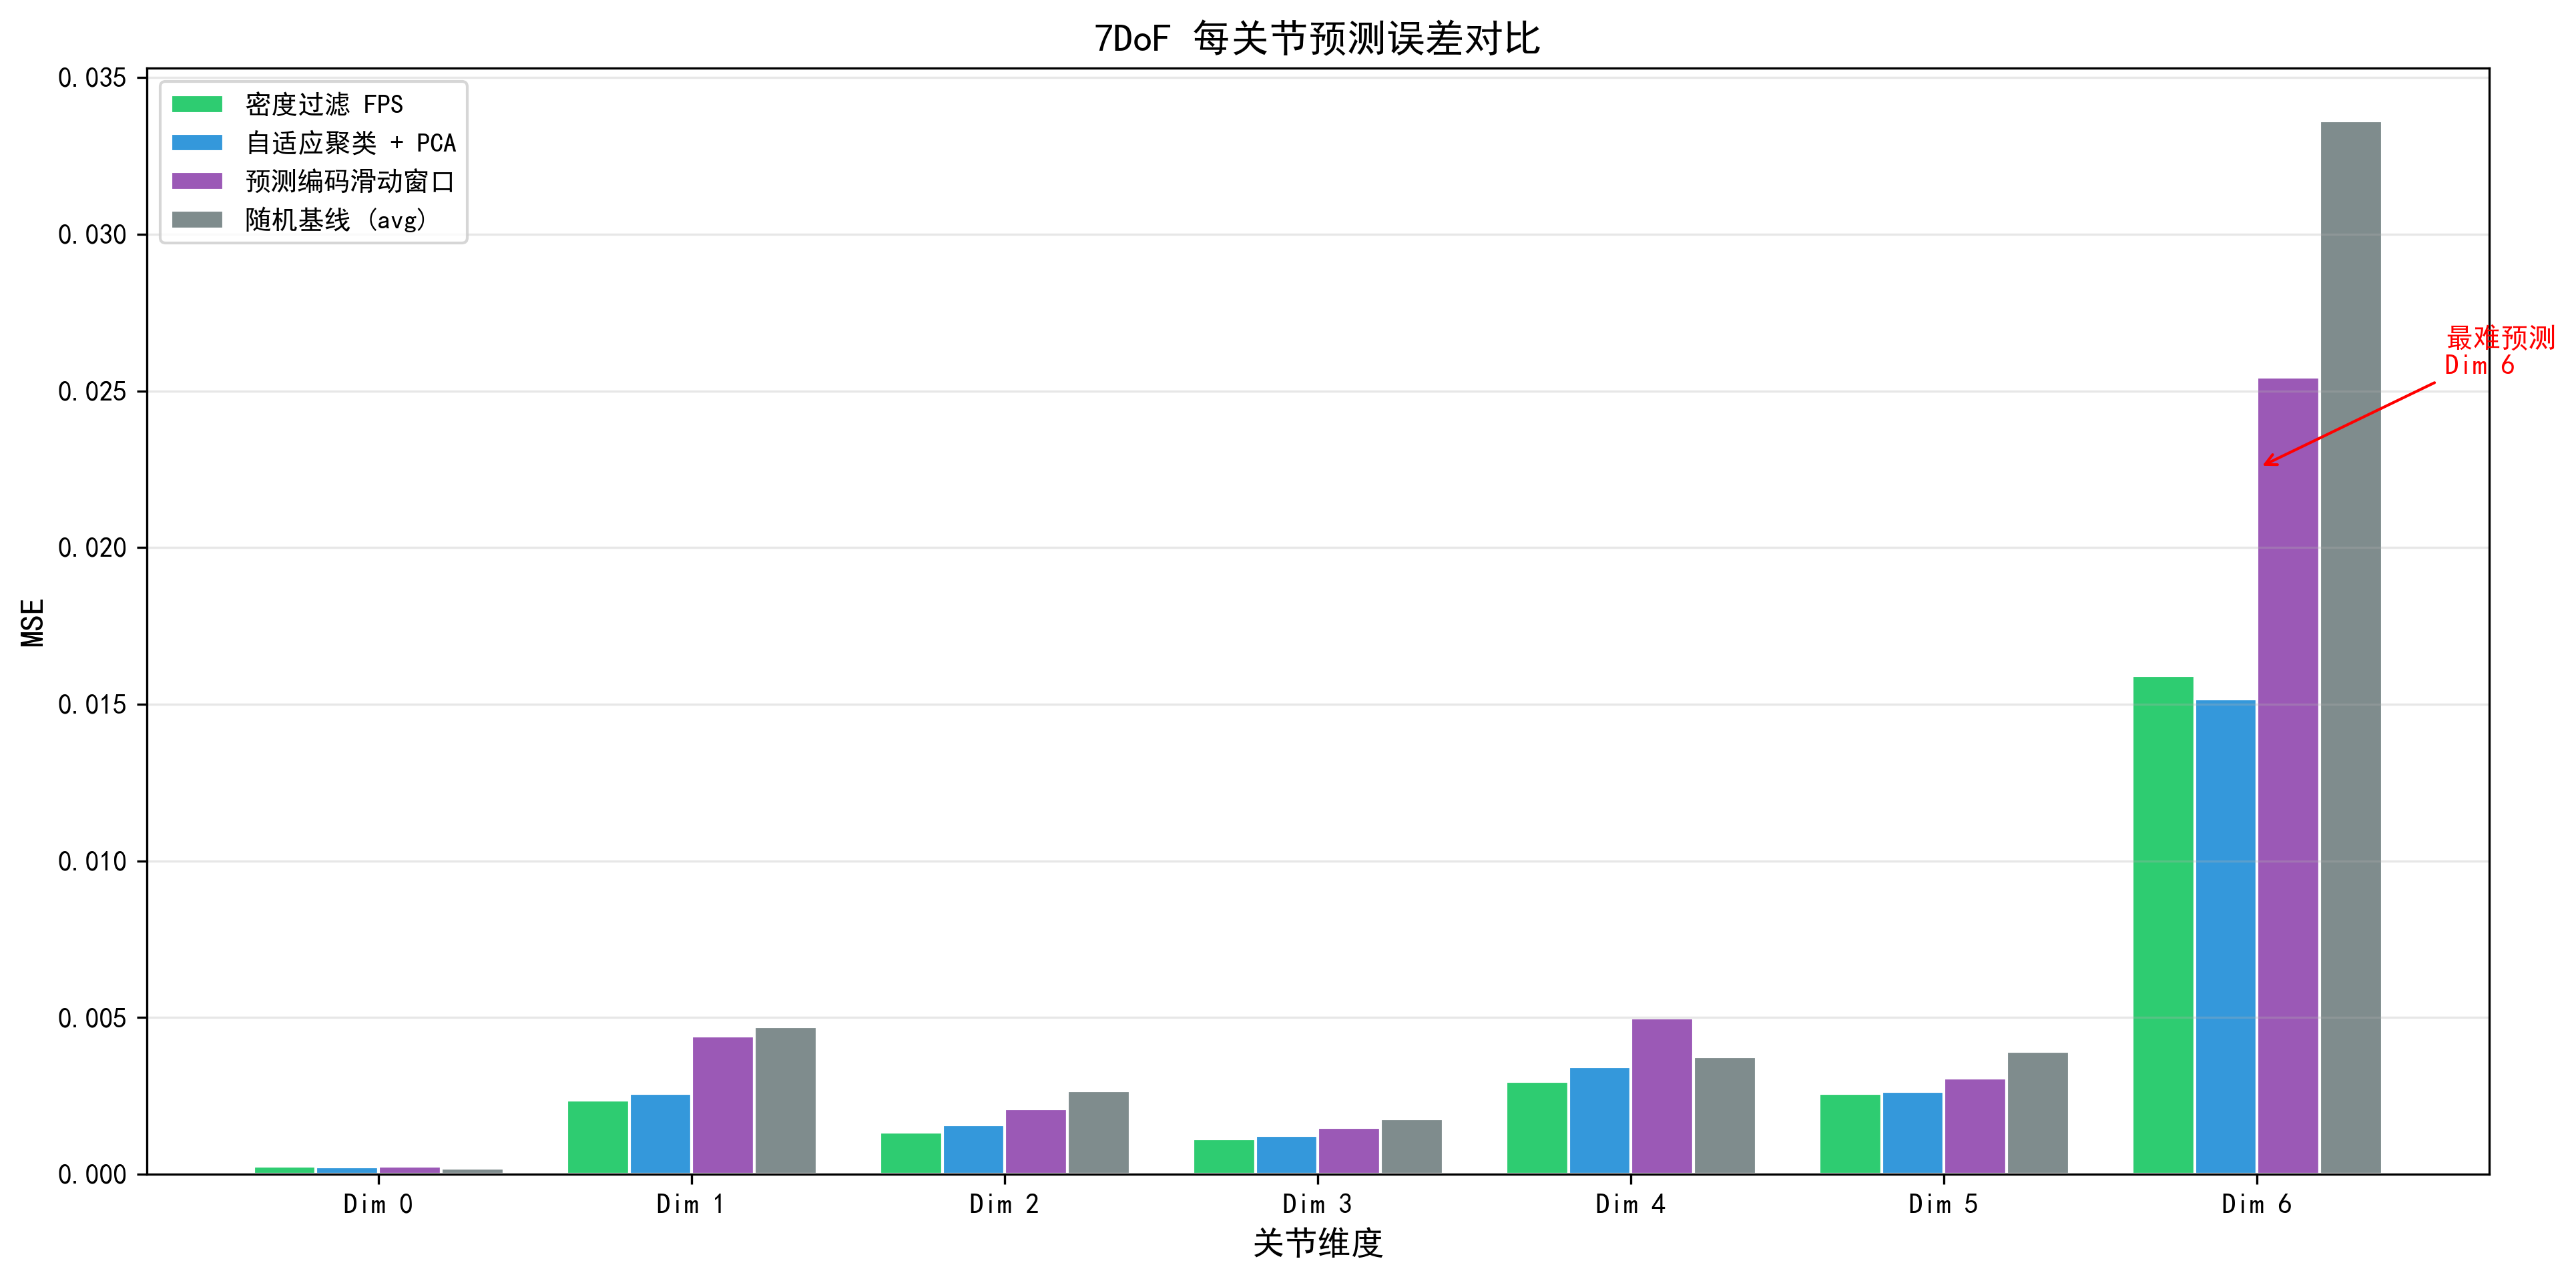
\includegraphics[width=0.95\textwidth]{fig6_dof_error}
    \caption{7DoF 每关节误差对比}
    \label{fig:dof_error}
\end{figure}

图~\ref{fig:dof_error}展示了四种方法在 7DoF 各关节上的 Test MSE 细粒度对比。最难预测维度为 gripper（夹爪开合），原因：夹爪开合是稀疏事件，随机采样容易遗漏。密度过滤 FPS 和自适应聚类筛选均显著改善 gripper 预测（$-$50\% 左右）。waist（腰部）绝对值极小，两种方法波动可忽略。shoulder 和 elbow 的大幅改善说明空间覆盖算法成功捕捉了手臂姿态的关键变化。

% ==================== 7. 结论与展望 ====================
\section{结论与展望}
\label{sec:conclusion}

\subsection{核心结论}

\begin{enumerate}[leftmargin=2em]
    \item \textbf{冗余没有普适定义，必须匹配数据特性与任务目标}。本文 5 种冗余定义中，分布冗余与几何覆盖冗余在单任务 CLIP 特征数据集上有效（MSE 降至 0.0038 量级），事件分割和压缩冗余失败（MSE 接近或高于随机基线），预测编码有效但有限（MSE 0.005688，降低 21.3\%）。这意味着：核心集选择算法的有效性首先取决于"冗余"这一概念的操作化定义是否与数据生成过程一致。
    
    \item \textbf{精准的直接操作优于复杂的层叠结构}。密度过滤 FPS 仅使用原始特征空间的距离计算和 k-NN 局部密度估计（2 层结构），即超越自适应聚类 + PCA 去噪的 3 层结构。预测编码滑动窗口同样证明了这一点：线性回归在 5 帧窗口内的直接预测（1 层结构）优于多尺度融合和联合得分的复杂层叠（MSE 0.005688 vs 0.006734）。
    
    \item \textbf{单一全局最优方法的信息完整性无法通过融合复现}。18 个融合实验（5 种架构 $\times$ 多种参数配置 + 预测编码 4 种改进尝试）全部失败。失败原因不是融合策略设计不够精巧，而是存在结构性瓶颈：信号不正交、信息漏斗效应、信息相关性上限。冗余信号必须是正交互补的，高度相关的信号融合只会放大噪声。
    
    \item \textbf{脑启发核心集选择可以显著提升数据效率}。在仅使用 10\% 训练数据的情况下，密度过滤 FPS 将 Test MSE 从随机基线的 0.007229 降至 0.003792，相对降低 47.5\%，证明了高质量子集对模仿学习的巨大价值。
\end{enumerate}

\subsection{局限性}

尽管密度过滤 FPS 在本文数据集上取得了最优性能，但本研究仍存在若干局限性，需要在后续工作中加以关注。

\textbf{首先，实验数据集的任务单一性可能限制了部分冗余定义的验证。}ALOHA Sim Transfer Cube 数据集仅包含"Transfer the cube"一项任务，场景、物体和相机视角相对固定。时序事件分割和自编码器重建误差等方法在如此规律的数据上难以展现优势，其失败可能部分源于数据多样性不足，而非方法本身无效。

\textbf{其次，语言指令的同质化限制了 CLIP 多模态特征的表达能力。}所有 Episode 共享相同的文本指令（"Transfer the cube"），导致文本特征无区分度，CLIP 的语义编码优势未能充分发挥。在多指令、多任务的设定下，基于文本-视觉对齐的冗余定义可能展现出不同的效果。

\textbf{第三，视觉输入仅依赖单一 top-down 视角，未利用多视角几何信息。}多视角一致性是判断遮挡、深度和物体姿态的重要线索，当前的核心集选择未能利用这一信息源。

\textbf{最后，核心集选择当前采用离线一次性计算，未探索在线增量更新机制。}在实际机器人学习场景中，数据流是持续到达的，如何在不重新计算全部选择的情况下增量更新核心集，是一个重要的工程问题。

\subsection{未来方向}

针对上述局限性与本文发现，未来研究可从以下几个方向展开。

\textbf{第一，在更大规模、多任务数据集上验证本文结论。}Open X-Embodiment 等跨机器人、跨任务数据集能够提供更丰富的场景多样性，有助于判断几何覆盖冗余是否仍能泛化，以及时序方法和 AE 方法是否在复杂任务中重新有效。

\textbf{第二，探索与空间覆盖真正正交的互补信号。}本文的融合实验表明，当前信号源高度相关，无法通过简单加权或分层产生信息增益。未来可引入模型不确定性、梯度范数、学习损失（learning loss）等主动学习指标，作为与几何覆盖互补的筛选维度。

\textbf{第三，设计可逆的分层核心集选择结构。}针对信息漏斗效应，未来可研究保留被过滤帧优先级信息的候选池机制，例如使用软注意力权重或优先级队列，使得精筛阶段能够恢复粗筛阶段误删的关键帧。

\textbf{第四，将核心集选择思想迁移至其他视觉任务。}例如，在雾天目标检测等场景中，可定义质量冗余、类别分布冗余、雾浓度分层冗余和视觉相似冗余等多重框架，验证核心集选择在不同任务结构中的适用性。

% ==================== 附录 ====================
\newpage
\appendix
\section{核心代码：四种核心集选择算法}
\label{app:code}

\subsection{A.1 自适应聚类 + PCA 核心集选择算法}

\textbf{思路}：分布冗余 —— 特征空间过度聚集的帧是冗余的。K-Means 聚类 + 稀疏簇偏好 + 动态保底 + PCA 400d 去噪。

\begin{minted}{python}
import numpy as np
from sklearn.cluster import KMeans
from sklearn.decomposition import PCA

class BrainInspiredCoresetSelector:
    """脑启发核心集选择器 v1.1 + PCA 400d"""
    def __init__(self, target_ratio=0.1, pca_components=400):
        self.target_ratio = target_ratio
        self.pca_components = pca_components
    
    def compute_diversity_scores(self, features, n_clusters=None):
        n = len(features)
        target_size = max(1, int(n * self.target_ratio))
        if n_clusters is None:
            n_clusters = max(2, target_size // 3)
        
        kmeans = KMeans(n_clusters=n_clusters, random_state=42, n_init=10)
        labels = kmeans.fit_predict(features)
        centers = kmeans.cluster_centers_
        
        dists = np.linalg.norm(features - centers[labels], axis=1)
        sizes = np.bincount(labels, minlength=n_clusters)
        size_penalty = 1.0 / np.sqrt(sizes[labels] + 1.0)
        scores = dists * size_penalty
        
        if scores.max() > scores.min():
            scores = (scores - scores.min()) / (scores.max() - scores.min() + 1e-8)
        return scores, labels
    
    def _get_cluster_quota(self, cluster_size):
        """动态保底：大簇多保底，小簇少保底"""
        return max(1, min(3, cluster_size // 50 + 1))
    
    def select(self, features, episode_indices, n_clusters=None):
        n = len(features)
        target_size = max(1, int(n * self.target_ratio))
        
        # PCA 400d 降维（仅用于聚类，不改变原始特征用于训练）
        pca = PCA(n_components=self.pca_components, random_state=42)
        features_pca = pca.fit_transform(features)
        
        scores, labels = self.compute_diversity_scores(features_pca, n_clusters)
        
        # 动态保底：按簇大小分配名额
        selected = set()
        for c in np.unique(labels):
            idx_in_c = np.where(labels == c)[0]
            quota = self._get_cluster_quota(len(idx_in_c))
            sorted_idx = idx_in_c[np.argsort(scores[idx_in_c])[-quota:]]
            for idx in sorted_idx:
                selected.add(int(idx))
        
        if len(selected) > target_size:
            selected = set(np.argsort(scores)[-target_size:])
        else:
            remaining = target_size - len(selected)
            if remaining > 0:
                unselected = [i for i in range(n) if i not in selected]
                top_local = np.argsort(scores[unselected])[-remaining:]
                for idx in top_local:
                    selected.add(unselected[idx])
        
        return np.array(sorted(list(selected)), dtype=np.int64)
\end{minted}

\subsection{A.2 密度过滤 FPS 核心集选择算法}

\textbf{思路}：几何覆盖冗余 —— "远且不孤立" = 最好。标准 FPS 保证空间覆盖，k-NN 局部密度过滤剔除孤立噪声点。

\begin{minted}{python}
import numpy as np
from sklearn.neighbors import NearestNeighbors

class DensityFilteredFPSSelector:
    """密度过滤最远点采样选择器"""
    def __init__(self, target_ratio=0.1, seed=42, k=5, filter_ratio=0.15):
        self.target_ratio = target_ratio
        self.seed = seed
        self.k = k
        self.filter_ratio = filter_ratio
    
    def select(self, features, actions, episode_indices):
        n = len(features)
        target_size = max(1, int(n * self.target_ratio))
        
        # Step 1: 标准 FPS 选出初始核心集
        from approaches.farthest_point_sampling.src.selector_fps import (
            FarthestPointSamplingSelector)
        fps = FarthestPointSamplingSelector(
            target_ratio=self.target_ratio, seed=self.seed)
        selected = fps.select(features, actions, episode_indices).tolist()
        
        # Step 2: 计算选中帧的局部密度（k-NN 平均距离）
        k = min(self.k, n - 1)
        nbrs = NearestNeighbors(n_neighbors=k + 1, algorithm='auto').fit(features)
        distances, _ = nbrs.kneighbors(features[selected])
        avg_dists = distances[:, 1:].mean(axis=1)
        
        # Step 3: 找出最低密度的 filter_ratio 比例
        n_replace = max(1, int(len(selected) * self.filter_ratio))
        replace_idx = np.argsort(avg_dists)[-n_replace:]
        
        # Step 4: 从全局未选帧中，找密度最高的帧替换
        unselected = [i for i in range(n) if i not in selected]
        if len(unselected) > 0:
            u_distances, _ = nbrs.kneighbors(features[unselected])
            u_avg_dists = u_distances[:, 1:].mean(axis=1)
            best_unselected = np.argsort(u_avg_dists)[:n_replace]
            for i, idx in enumerate(replace_idx):
                if i < len(best_unselected):
                    selected[idx] = unselected[best_unselected[i]]
        
        return np.array(sorted(selected), dtype=np.int64)
\end{minted}

\subsection{A.3 预测编码滑动窗口核心集选择算法}

\textbf{思路}：时序冗余 —— 可预测 = 冗余。在每个 episode 内用滑动窗口自回归预测当前帧动作，预测残差大的帧 = 打破预测 = 高价值。

\begin{minted}{python}
import numpy as np

class PredictiveCodingSelector:
    """滑动窗口自回归预测编码选择器"""
    def __init__(self, target_ratio=0.1, window=5, seed=42):
        self.target_ratio = target_ratio
        self.window = window
        self.seed = seed
    
    def _compute_residuals(self, actions, episode_indices):
        n = len(actions)
        residuals = np.zeros(n)
        
        for ep in np.unique(episode_indices):
            mask = episode_indices == ep
            idx = np.where(mask)[0]
            ep_actions = actions[idx]
            n_ep = len(ep_actions)
            
            if n_ep <= self.window + 1:
                residuals[idx] = 1e6
                continue
            
            X_list, y_list = [], []
            for t in range(self.window, n_ep):
                X_list.append(ep_actions[t - self.window:t].flatten())
                y_list.append(ep_actions[t])
            
            X_win = np.array(X_list)
            y_tgt = np.array(y_list)
            
            XtX = X_win.T @ X_win
            Xty = X_win.T @ y_tgt
            reg = 1e-6 * np.eye(XtX.shape[0])
            w = np.linalg.solve(XtX + reg, Xty)
            
            y_pred = X_win @ w
            errors = np.mean((y_pred - y_tgt) ** 2, axis=1)
            
            residuals[idx[:self.window]] = 1e6
            residuals[idx[self.window:]] = errors
        
        return residuals
    
    def select(self, features, actions, episode_indices):
        n = len(actions)
        target_size = max(1, int(n * self.target_ratio))
        
        prediction_errors = self._compute_residuals(actions, episode_indices)
        selected_idx = np.argsort(prediction_errors)[-target_size:]
        
        return np.array(sorted(selected_idx), dtype=np.int64)
\end{minted}

\subsection{A.4 分层融合核心集选择算法}

\textbf{思路}：分层融合 —— v1.1 负责语义粗筛，FPS 负责几何精筛。最佳融合思路（MSE 0.004004），但仍未超越单一最优。

\begin{minted}{python}
import numpy as np

class HierarchicalFusionSelector:
    """分层融合选择器 v2.0：v1.1 粗筛 + FPS 精筛"""
    def __init__(self, target_ratio=0.1, candidate_ratio=2.0,
                 pca_components=400, seed=42):
        self.target_ratio = target_ratio
        self.candidate_ratio = candidate_ratio
        self.pca_components = pca_components
        self.seed = seed
    
    def select(self, features, actions, episode_indices):
        n = len(features)
        target_size = max(1, int(n * self.target_ratio))
        
        # Layer 1: v1.1 + PCA 400d 粗筛候选池
        v1_ratio = min(1.0, self.target_ratio * self.candidate_ratio)
        from approaches.redundancy_distribution.src.selector_v1_1_pca_best import (
            BrainInspiredCoresetSelector as V1Selector)
        v1_selector = V1Selector(
            target_ratio=v1_ratio, pca_components=self.pca_components)
        fixed_n_clusters = max(10, len(features) // 30)
        candidates = v1_selector.select(features, episode_indices,
                                         n_clusters=fixed_n_clusters)
        
        # Layer 2: FPS 在候选池内精筛
        pool_size = len(candidates)
        fps_ratio = target_size / pool_size
        from approaches.farthest_point_sampling.src.selector_fps import (
            FarthestPointSamplingSelector)
        fps_selector = FarthestPointSamplingSelector(
            target_ratio=fps_ratio, seed=self.seed)
        fps_local_idx = fps_selector.select(
            features[candidates], actions[candidates],
            episode_indices[candidates])
        
        selected = candidates[fps_local_idx]
        return np.array(sorted(selected), dtype=np.int64)
\end{minted}

% ==================== 参考文献 ====================
\begin{thebibliography}{99}
\bibitem{zhao2023act}
Zhao T, et al. Learning Fine-Grained Bimanual Manipulation with Low-Cost Hardware. \textit{RSS}, 2023.

\bibitem{sorscher2022beyond}
Sorscher B, et al. Beyond neural scaling laws: beating power law scaling via data pruning. \textit{NeurIPS}, 2022.

\bibitem{kim2024openvla}
Kim K, et al. OpenVLA: An Open-Source Vision-Language-Action Model. \textit{arXiv:2406.09246}, 2024.

\bibitem{radford2021clip}
Radford A, et al. Learning Transferable Visual Models From Natural Language Supervision. \textit{ICML}, 2021.

\bibitem{he2016resnet}
He K, et al. Deep Residual Learning for Image Recognition. \textit{CVPR}, 2016.

\bibitem{millidge2021predictive}
Millidge A, et al. Predictive coding: a theoretical and experimental review. \textit{arXiv:2107.12979}, 2021.
\end{thebibliography}

\end{document}
